\documentclass[12pt,a4paper,oneside]{report}

\usepackage[utf8]{inputenc}
\usepackage[T1]{fontenc}
\usepackage{lmodern}
\usepackage{geometry}
\usepackage{setspace}
\usepackage{microtype}
\usepackage{amsmath,amssymb}
\usepackage{booktabs}
\usepackage{longtable}
\usepackage{tabularx}
\usepackage{array}
\usepackage{graphicx}
\usepackage{float}
\usepackage{caption}
\usepackage{subcaption}
\usepackage{enumitem}
\usepackage{xcolor}
\usepackage{url}
\usepackage{xurl}
% Parenthetical author--year citations; full names in the reference list.
\usepackage[authoryear,round]{natbib}
\setcitestyle{authoryear,round,aysep={,},citesep={;}}
\usepackage[hidelinks]{hyperref}
\newcommand{\doi}[1]{doi:\space\href{https://doi.org/#1}{\begingroup\urlstyle{rm}\nolinkurl{#1}\endgroup}}
\usepackage{fancyhdr}

\geometry{left=1.25in,right=1in,top=1in,bottom=1in}
\onehalfspacing
\setlength{\parindent}{0.5in}
\setlength{\parskip}{0.25em}
\setlength{\emergencystretch}{2em}
\setcounter{secnumdepth}{3}
\setcounter{tocdepth}{2}

\pagestyle{fancy}
\fancyhf{}
\fancyhead[L]{Deltx Research Project}
\fancyhead[R]{\thepage}
\renewcommand{\headrulewidth}{0.4pt}
\setlength{\headheight}{15pt}

\newcommand{\systemname}{\textsc{Deltx}}
\newcommand{\code}[1]{\nolinkurl{#1}}
\newcommand{\pending}{\textit{To be inserted from the completed forecasting experiment outputs.}}
\newcolumntype{Y}{>{\raggedright\arraybackslash}X}
\newcolumntype{P}[1]{>{\raggedright\arraybackslash}p{#1}}

\newcommand{\repovis}[5]{%
\begin{figure}[p]
    \centering
    \begin{subfigure}{0.96\textwidth}
        \centering
        \includegraphics[width=\textwidth,height=0.30\textheight,keepaspectratio]{#2}
        \caption{Commit-sequence score variation.}
    \end{subfigure}

    \vspace{0.4cm}
    \begin{subfigure}{0.47\textwidth}
        \centering
        \includegraphics[width=\textwidth,height=0.25\textheight,keepaspectratio]{#3}
        \caption{Correlation heatmap.}
    \end{subfigure}\hfill
    \begin{subfigure}{0.47\textwidth}
        \centering
        \includegraphics[width=\textwidth,height=0.25\textheight,keepaspectratio]{#4}
        \caption{Pairwise scatter visualization.}
    \end{subfigure}
    \caption{Exploratory Deltx dataset visualizations for #1. These figures are the supplied visualization outputs generated from the extracted repository dataset.}
    \label{fig:#5}
\end{figure}
}

\begin{document}

\hypersetup{pageanchor=false}
\begin{titlepage}
    \centering
    \vspace*{1.2cm}

    {\Large \textbf{Deltx: An Intelligent Static Analysis and Predictive Analytics Platform for Software Quality Evolution}\par}
    \vspace{1.0cm}
    {\LARGE \textbf{Interim Research Report}\par}

    \vspace{1.8cm}

    \begin{tabular}{ll}
        \textbf{S.M. Silva} & Index No: 22001905 \\
        \textbf{Praneesh S.} & Index No: 22001591 \\
        \textbf{R.M.I.M. De Silva} & Index No: 22000331 \\
    \end{tabular}

    \vspace{1.5cm}

    \textbf{Supervisor}\\[0.25cm]
    Dr. Manjusri Wickramasinghe

    \vfill

    {\large University of Colombo School of Computing\par}
    {\large Colombo, Sri Lanka\par}
    \vspace{0.5cm}
    {\large October 2026\par}
\end{titlepage}

\pagenumbering{roman}
\hypersetup{pageanchor=true}

\chapter*{List of Acronyms}
\addcontentsline{toc}{chapter}{List of Acronyms}
\begin{longtable}{p{0.20\textwidth}p{0.72\textwidth}}
AI & Artificial Intelligence \\
AST & Abstract Syntax Tree \\
CI/CD & Continuous Integration and Continuous Deployment \\
ECDF & Empirical Cumulative Distribution Function \\
GRU & Gated Recurrent Unit \\
LLM & Large Language Model \\
LSTM & Long Short-Term Memory \\
LTSF & Long-Term Time Series Forecasting \\
MAE & Mean Absolute Error \\
MLP & Multilayer Perceptron \\
MQR & Multi-Quality Rule mode in SonarQube \\
NCLOC & Non-comment Lines of Code \\
PatchTST & Patch Time Series Transformer \\
RMSE & Root Mean Square Error \\
SHAP & SHapley Additive exPlanations \\
SQUALE & Software QUALity Enhancement \\
XAI & Explainable Artificial Intelligence \\
\end{longtable}

\tableofcontents
\clearpage
\pagenumbering{arabic}

% =============================================================================
\chapter{Introduction}
\label{ch:introduction}
% =============================================================================

\section{Background and Motivation}
The software engineering landscape is undergoing a major shift driven by the adoption of Large Language Models (LLMs) and AI-assisted programming agents. AI-assisted development can accelerate implementation, but it also changes how software is produced and can introduce structural vulnerabilities, architectural inconsistencies, latent technical debt, and other risks that may only become visible as the codebase evolves. Existing empirical work reports measurable differences between human-written and AI-generated code in defects, vulnerabilities, and complexity \citep{human_written_vs_ai_generated_code_2025}. Limited self-declaration of AI involvement in real repositories makes it difficult to study its longitudinal effect on software quality \citep{developers_self_declaration_ai_generated_code}.

Software quality is described at a high level by standards such as ISO/IEC 25010, while static-analysis platforms such as SonarQube provide operational measurements and rule violations. However, static analysis is fundamentally retrospective: it reports the current condition of a codebase rather than predicting how software quality may evolve in future commits.

\section{Problem Statement and Research Gaps}

\subsection{Issue 1: Invisibility of AI-Generated Structural Decay}
Current static-analysis tools process source code without distinguishing human-authored code from AI-generated code. AI-generated code can be functionally correct in isolation while introducing structural problems when integrated into a larger codebase. Without an authorship signal, organizations cannot separately observe the evolution of AI-assisted code or study whether changes in AI-authorship are associated with later quality degradation.

\subsection{Issue 2: Semantic Gap in Software Quality Metrics}
SonarQube produces granular rule violations and structural measurements, but there is a semantic gap between these low-level outputs and higher-level software-quality dimensions such as Correctness, Maintainability, Security, and Efficiency. Simple counting or arithmetic aggregation can also mask severe problems when many less important observations are present. \systemname{} uses SQUALE-style nonlinear aggregation to address this conflict-resistance requirement \citep{squale_model_practice_based_industrial_quality_model,software_quality_metrics_aggregation_industry}.

\subsection{Issue 3: Retrospective Nature of Static Analysis}
Static-analysis platforms provide point-in-time snapshots but do not directly forecast how quality will evolve across future commits. This leaves software teams in a reactive position, where degradation is addressed only after it has already appeared. \systemname{} addresses this by constructing chronological repository-quality histories that can be used for multivariate time-series forecasting.

\subsection{Issue 4: Lack of Interpretability in Predictive Metrics}
Predictive models can be difficult for developers to trust when they provide only numerical forecasts. If the system predicts a future decline in Maintainability, Correctness, Security, or Efficiency, developers need an explanation of which historical variables and time periods influenced that forecast. The planned interpretation layer therefore uses SHAP-based feature attribution \citep{perspective_on_xai_methods_shap_and_lime}.

\section{Scope}
The project scope is intentionally restricted to Python repositories. The current research pipeline consists of five stages: repository-history extraction, AI-authorship detection, SQUALE-based quality aggregation, multivariate time-series forecasting, and SHAP-based interpretation. The first three stages are implemented. Forecasting experiments have begun using datasets extracted from multiple repositories, while the final interpretation layer remains planned.

Commits that contain no meaningful Python syntax change are excluded using AST-based semantic comparison; documentation-only, comment-only, docstring-only, whitespace-only, formatting-only, and equivalent-rename commits are filtered.

\section{Research Aim}
The research aim is to conceptualize, design, and evaluate \systemname{}, an architecture integrating static code analysis, AI detection, predictive modeling, and explainability in order to transform retrospective software-quality measurements into proactive quality trajectories.

\section{Current Progress}
Table~\ref{tab:progress} summarizes the interim implementation state.

\begin{table}[H]
\centering
\caption{Current implementation progress.}
\label{tab:progress}
\begin{tabularx}{\textwidth}{p{0.08\textwidth}p{0.31\textwidth}p{0.24\textwidth}Y}
\toprule
\textbf{Stage} & \textbf{Module} & \textbf{Status} & \textbf{Current state} \\
\midrule
1 & \code{deltx.extraction} & Implemented & Python history extraction, semantic checkpoint filtering, churn, topology, dataset orchestration. \\
2 & \code{deltx.detection} & Implemented & DroidDetect-Base-Binary inference with file/chunk aggregation to \code{ai\_confidence\_pct}. \\
3 & \code{deltx.scoring} & Implemented & Dockerized SonarQube analysis, modern MQR mappings, dynamic issue weighting, SQUALE-based four-score aggregation. \\
4 & \code{deltx.prediction} & Experimental & Multiple forecasting models have been trained; final comparative results are to be inserted from the experiment outputs. \\
5 & \code{deltx.interpretation} & Planned & SHAP-based explanation of the selected forecasting model. \\
\bottomrule
\end{tabularx}
\end{table}

% =============================================================================
\chapter{Literature Review}
\label{ch:literature}
% =============================================================================

The theoretical foundation is organized around four domains: AI-generated code detection, hierarchical software-quality modeling, predictive time-series modeling, and Explainable Artificial Intelligence.

\section{AI-Generated Text and Code Detection}
The growing use of LLMs has motivated methods for distinguishing synthetic content from human authorship. Earlier approaches often depended on perplexity, token likelihoods, or related statistical signatures.

The project uses the published DroidDetect-Base-Binary checkpoint from the Droid resource suite \citep{orel2025droid}. The detector is fine-tuned from ModernBERT-base and covers Python among its supported languages. The binary head separates human-generated and machine-generated code, where the machine-generated class includes generated, refined, and adversarial examples. \systemname{} does not train a new detector; it uses the published detector as an authorship signal and aggregates file-level outputs into a commit-level score.

The current score is
\begin{equation}
    \mathrm{ai\_confidence\_pct}=100\left(1-P(\mathrm{HUMAN\_GENERATED})\right).
\end{equation}
The detector output is treated as an ordinal confidence signal rather than a calibrated probability. The implementation also preserves full-file context where possible because fragment-level evaluation was observed to produce substantially higher false-positive behavior in local verification.

\section{Hierarchical Software Quality Models}
ISO/IEC 25010 provides a high-level vocabulary for software quality, but operational tools produce low-level measurements and rule violations. Bridging this abstraction gap is a long-standing software-engineering problem. The Quamoco approach formalized mappings between concrete measurements and quality factors \citep{quamoco_product_quality_modelling_assessment}. SQUALE provides a practice-based quality model that normalizes heterogeneous observations into marks and aggregates them using nonlinear functions that give greater influence to poor values \citep{squale_model_practice_based_industrial_quality_model,software_quality_metrics_aggregation_industry}.

These quality models inform the scoring methodology. \systemname{} uses SonarQube as the measurement instrument and SQUALE-inspired nonlinear aggregation as the mechanism for converting granular findings into four continuous target scores. Current SonarQube MQR findings can carry separate Maintainability, Reliability, and Security impacts, and the implemented scoring model preserves those multi-impact semantics rather than collapsing an issue to a single legacy type.

\section{Predictive Time-Series Modeling}
Historical software-quality measurements support fault prediction and quality forecasting \citep{fault_prediction_software_metrics_sonarqube_rules,software_service_supporting_software_quality_forecasting}. Relevant candidates include LSTM and GRU networks \citep{chung2014gated_recurrent_networks}, LTSF-Linear models \citep{zeng2023ltsf_linear}, PatchMLP \citep{tang2024patchmlp}, and PatchTST \citep{nie2023patchtst}.

\systemname{} will compare these candidates using repository histories containing the four quality scores alongside AI-authorship, churn, structural, and static-analysis features. The final model will be selected according to MAE and RMSE on validation data, with separate evaluation of its ability to generalize to unseen repositories.

\section{Explainable Artificial Intelligence}
The final research component is explainability. SHAP uses Shapley-value principles to quantify the contribution of input variables to a model prediction \citep{perspective_on_xai_methods_shap_and_lime}. Within \systemname{}, SHAP is intended to explain the forecasting model rather than source-code semantics directly. A predicted decline can therefore be traced to historical channels such as changes in quality scores, AI confidence, churn, centrality, issue densities, complexity, or duplication.

% =============================================================================
\chapter{Research Objectives / Questions}
\label{ch:objectives}
% =============================================================================

\section{Research Objectives}
\begin{enumerate}[leftmargin=*,label=\textbf{\arabic*.}]
    \item \textbf{AI Code Detection Methodology.} To operationalize an AI Code Detection methodology using the published DroidDetect-Base-Binary detector to estimate AI-authorship confidence for newly introduced Python code and aggregate detector outputs, weighted by the number of code lines, into a commit-level AI-authorship signal.

    \item \textbf{Quality Mapping and Weighting Mechanism.} To formulate a mapping and weighting mechanism that translates granular SonarQube rule violations into four primary ISO/IEC 25010 dimensions (Maintainability, Correctness, Security, Efficiency), explicitly factoring in issue severity, occurrence frequency, code churn, and call-graph centrality.

    \item \textbf{Conflict-Resistant Quality Scoring System.} To engineer a conflict-resistant Quality Scoring System, inspired by hierarchical frameworks such as SQUALE, that computes normalized scores on a 0--100 scale for each overarching quality dimension, with explicit penalization of outliers.

    \item \textbf{Predictive Modeling and Model Selection.} To compare forecasting models using multivariate historical metric time series and select the best-performing model for forecasting future quality-score trajectories with statistically robust confidence intervals.

    \item \textbf{Interpretation Layer with SHAP Integration.} To integrate a comprehensive Interpretation Layer utilizing SHAP methodologies to translate numerical quality forecasts into semantic, human-readable insights, benchmarked against empirically derived industry thresholds.

    \item \textbf{Dataset Construction and Empirical Foundation.} To design and construct a temporally structured, chronologically mined dataset from mature open-source Python repositories, pairing probabilistic AI-authorship signals with continuous SonarQube quality metrics at discrete commit checkpoints, to serve as the empirical foundation for training and evaluating the predictive modeling engine.
\end{enumerate}

% =============================================================================
\chapter{Research Approach and Methodology}
\label{ch:methodology}
% =============================================================================

\section{System Architecture Overview}
\systemname{} is designed to study how AI-assisted development relates to changes in software quality over time in Python projects. The work is divided into five stages that can be assessed separately and together.

\begin{enumerate}[leftmargin=*]
    \item Extract meaningful Python checkpoints and repository-evolution features.
    \item Compute a commit-level AI-authorship confidence signal using the existing detector.
    \item Scan each Python snapshot with SonarQube and convert issues/measures to four SQUALE-based quality targets.
    \item Construct time-series windows and train forecasting models.
    \item Explain selected forecasts using SHAP.
\end{enumerate}

\section{Dataset Construction and Checkpoint Selection}
The dataset represents repository evolution as a chronological sequence of checkpoints, with one observation for each commit that introduces a meaningful change to Python source code. Changes are identified by comparing each non-root commit with its \textbf{first parent}; the root commit is compared with an empty repository state. Restricting the analysis to Python provides a consistent basis for authorship and software-quality measurements within a single programming language.

Checkpoint selection uses abstract syntax tree (AST) comparison to distinguish changes in program structure from changes that leave the normalized syntax representation unchanged. The following commit types are excluded:
\begin{itemize}
    \item commits that change only non-Python files such as README files, documentation, images, configuration files, lock files, or other assets;
    \item Python changes that add or modify only comments;
    \item Python changes that modify only recognized module, class, function, or asynchronous-function docstrings;
    \item whitespace-only and formatting-only Python changes;
    \item pure Python-file renames whose normalized program contents are unchanged; and
    \item other changes whose normalized Python syntax is semantically unchanged under the AST-based comparison.
\end{itemize}

The selected repository states are examined as historical snapshots. For each checkpoint, code churn is measured from Python lines added and deleted relative to the first parent. Structural impact is represented by an import-dependency graph, in which nodes correspond to Python files and edges represent imports within the repository. PageRank provides a centrality measure that is included as a dataset feature and used to account for the structural importance of affected files during issue weighting.

\section{AI Authorship Detection Methodology}
The current implementation uses DroidDetect-Base-Binary from the Droid resource suite \citep{orel2025droid}. For each non-root checkpoint, Deltx compares the commit with its \textbf{first parent} and scopes authorship detection to the \textbf{new Python code introduced by that commit}. Unchanged pre-existing code is excluded from this authorship measurement, and deleted code has no current content to classify. This makes \code{ai\_confidence\_pct} an authorship signal for the code being introduced at that evolution step rather than a score for the entire repository state.

The rationale for this scope is that integrating newly written code into an existing repository does not change whether that code was human- or AI-authored. AI authorship is therefore measured on the newly introduced code itself. The resulting code-level probabilities are aggregated using a code-line-weighted average to obtain the commit-level \code{ai\_confidence\_pct} in the range 0--100, which occupies numeric feature index~4.

A probabilistic AI-authorship signal is produced independently from the quality-scoring engine. The AI signal is not used as a penalty in SQUALE; it serves as an evolutionary driver for the forecasting stage.

\section{Repository Quality Assessment}
At each selected checkpoint, SonarQube analyzes the \textbf{complete Python repository snapshot} to assess software quality after the commit. This captures issues in newly introduced code and those arising from its interaction with the existing codebase. The findings are aggregated using SQUALE to obtain repository-level Maintainability, Correctness, Security, and Efficiency scores.

Measurements include NCLOC, cognitive complexity, duplicated-lines density, and maintainability remediation effort. Issue weighting incorporates file centrality, measured using PageRank over the Python import graph, and historical file volatility derived from earlier commits. Missing measures are treated as unavailable rather than as zero. The SonarQube version and quality-profile configuration are recorded for reproducibility.

The dataset combines \textbf{AI confidence for newly introduced Python code} with \textbf{quality scores for the complete repository state}. Quality changes associated with a commit are assessed by comparing its scores with those of its first parent.

\section{Quality Mapping}
The implemented mapping is:
\begin{align*}
\mathrm{MAINTAINABILITY} &\rightarrow \mathrm{score\_maintainability},\\
\mathrm{RELIABILITY} &\rightarrow \mathrm{score\_correctness},\\
\mathrm{SECURITY} &\rightarrow \mathrm{score\_security}.
\end{align*}
A single Sonar issue can affect more than one quality, and each quality retains its own severity. For Efficiency, SonarQube does not expose a dedicated software quality. Deltx therefore uses active Python rules whose authoritative Clean Code attribute is \code{EFFICIENT}. This is additive: an issue can influence Reliability/Correctness and Efficiency simultaneously. The Efficiency score is a static-analysis-derived proxy and must not be interpreted as direct runtime performance measurement.

\section{Dynamic Issue Weighting}
For a rule count at checkpoint $t$, the issue density and bounded frequency signal are
\begin{align}
\mathrm{density}(r,t) &= \frac{\mathrm{count}(r,t)}{\max(\mathrm{NCLOC}_t,1)}\times1000,\\
F'(r,t) &= \frac{\ln(1+\mathrm{density})}{1+\ln(1+\mathrm{density})}.
\end{align}
For a file $f$, centrality is represented by the within-repository empirical percentile of its PageRank:
\begin{equation}
C'(f,t)=\mathrm{ECDF}(PR(f,t)).
\end{equation}
Historical volatility is
\begin{equation}
V(f,t)=\sum_{k=1}^{H}\delta^{k-1}\frac{\mathrm{added}(f,t-k)+\mathrm{deleted}(f,t-k)}{\max(\mathrm{previous\_loc}(f,t-k),1)},
\end{equation}
with bounded transform
\begin{equation}
CH'(f,t)=\frac{\ln(1+V)}{1+\ln(1+V)}.
\end{equation}
The dynamic weight for issue $i$ mapped to quality dimension $d$ is
\begin{equation}
W(i,d,t)=M(i,d)S(i,d)\left[1+\rho_d\left(\alpha_dF'_i+\beta_dC'_i+\gamma_dCH'_i\right)\right].
\end{equation}
The current research baseline uses equal $\alpha$, $\beta$, and $\gamma$ values of $1/3$, with $\rho=1$. These are provisional baseline values and not validated Python-optimal parameters.

\section{Individual Marks and SQUALE Aggregation}
The issue weight is converted to a common 0--3 mark:
\begin{equation}
IM(i,d)=3\left[1-\mathrm{clip}\left(\frac{W}{5(1+\rho_d)},0,1\right)^{\kappa_d}\right].
\end{equation}
For individual marks $IM_j$ and positive aggregation weights $\omega_j$, Deltx uses
\begin{equation}
M_d=-\frac{\ln\left(\frac{\sum_j\omega_j\lambda_d^{-IM_j}}{\sum_j\omega_j}\right)}{\ln(\lambda_d)},
\end{equation}
followed by
\begin{equation}
\mathrm{score}_d=\mathrm{clip}\left(\frac{100}{3}M_d,0,100\right).
\end{equation}
The exponential mean gives lower marks greater influence than arithmetic averaging, reducing the extent to which higher marks can compensate for poorer quality.

\section{Maintainability Composite}
Maintainability is not based only on issue impacts. First, all MAINTAINABILITY issue marks are aggregated into a 0--3 issue-practice mark. Three additional project-level practices are transformed using
\begin{equation}
\mathrm{metric\_mark}(x)=\frac{3}{1+(x/\tau)^k}.
\end{equation}
The four outer practices are:
\begin{enumerate}[leftmargin=*]
    \item the aggregated MAINTAINABILITY issue-practice mark;
    \item technical debt per KLOC, $\mathrm{sqale\_index}/\max(\mathrm{NCLOC},1)\times1000$;
    \item cognitive complexity per KLOC;
    \item duplicated-lines density, used directly because it is already normalized.
\end{enumerate}
These four practice marks are then combined with the nonlinear SQUALE aggregation to obtain \code{score\_maintainability}. The current baseline uses $\lambda=9$, debt threshold $\tau=1000$ minutes/KLOC, complexity threshold $\tau=100$ per KLOC, and duplication threshold $\tau=5\%$, with unit shape/aggregation weights. These are research baselines rather than empirically validated thresholds.

\section{Dataset Vector}
Each generated CSV row begins with the two identifiers \code{repository} and \code{commit\_hash}, followed by the 15 numeric features in Table~\ref{tab:vector}. The identifiers are used for grouping and traceability and are excluded from model inputs.

\small
\begin{longtable}{@{}P{0.08\textwidth}P{0.20\textwidth}P{0.28\textwidth}P{\dimexpr0.44\textwidth-6\tabcolsep\relax}@{}}
\caption{Deltx commit-level data vector.}\label{tab:vector}\\
\toprule
\textbf{Index} & \textbf{Classification} & \textbf{Variable} & \textbf{Description} \\
\midrule
\endfirsthead
\toprule
\textbf{Index} & \textbf{Classification} & \textbf{Variable} & \textbf{Description} \\
\midrule
\endhead
-- & Identifier & \code{repository} & Repository directory name used for grouping and traceability. \\
-- & Identifier & \code{commit\_hash} & Full Git commit object identifier. \\
0 & Predictive Target & \code{score\_maintainability} & SQUALE score using MAINTAINABILITY impacts plus debt/KLOC, cognitive complexity/KLOC, and duplication density. \\
1 & Predictive Target & \code{score\_correctness} & SQUALE score from Sonar RELIABILITY impacts. \\
2 & Predictive Target & \code{score\_security} & SQUALE score from Sonar SECURITY impacts. \\
3 & Predictive Target & \code{score\_efficiency} & SQUALE score from active Python rules with Clean Code attribute \code{EFFICIENT}. \\
4 & Evolutionary Driver & \code{ai\_confidence\_pct} & LOC-weighted commit-level AI authorship confidence in $[0,100]$. \\
5 & Evolutionary Driver & \code{loc\_added} & Python lines added in the checkpoint. \\
6 & Evolutionary Driver & \code{loc\_deleted} & Python lines deleted in the checkpoint. \\
7 & Evolutionary Driver & \code{files\_modified\_count} & Number of modified Python files. \\
8 & Topological Impact & \code{avg\_pagerank\_centrality} & Mean raw PageRank of meaningfully changed Python files. \\
9 & Static Analysis Signal & \code{density\_blocker\_issues} & Blocker issue density per KLOC. \\
10 & Static Analysis Signal & \code{density\_critical\_issues} & Critical/high issue density per KLOC under the fixed dataset bucket mapping. \\
11 & Static Analysis Signal & \code{density\_major\_issues} & Major/medium issue density per KLOC. \\
12 & Static Analysis Signal & \code{density\_minor\_issues} & Minor/low issue density per KLOC. \\
13 & Static Analysis Signal & \code{cognitive\_complexity} & Sonar project cognitive complexity. \\
14 & Static Analysis Signal & \code{duplication\_density} & Sonar duplicated-lines density percentage. \\
\bottomrule
\end{longtable}
\normalsize

\section{Predictive Modeling and Interpretation}
Forecasting uses historical windows of the 15 numeric channels and predicts future values of the four target scores. Repository identifiers are used to prevent windows from crossing repository boundaries. Time-aware splitting is required so future checkpoints are not exposed to training through overlapping windows. The final selected forecasting model will be interpreted using SHAP to identify the historical channels and time windows that contribute most strongly to each forecast.

% =============================================================================
\chapter{Experiments and Preliminary Results}
\label{ch:results}
% =============================================================================

\section{Repositories Analysed}
At the current interim stage, datasets have been extracted from the 15 Python repositories listed in Table~\ref{tab:repos}. The table also summarizes the role of each repository and the size of its public commit history.

\begingroup
\footnotesize
\setlength{\tabcolsep}{3pt}
\begin{longtable}{@{}P{0.05\textwidth}P{0.15\textwidth}P{0.33\textwidth}>{\raggedleft\arraybackslash}p{0.11\textwidth}P{\dimexpr0.36\textwidth-8\tabcolsep\relax}@{}}
\caption{Repositories currently analysed with the Deltx data pipeline.}\label{tab:repos}\\
\toprule
\textbf{No.} & \textbf{Repository} & \textbf{Repository type / purpose} & \textbf{Commits} & \hspace{0.5em}\textbf{Source} \\
\midrule
\endfirsthead
\toprule
\textbf{No.} & \textbf{Repository} & \textbf{Repository type / purpose} & \textbf{Commits} & \hspace{0.5em}\textbf{Source} \\
\midrule
\endhead
1 & Pyevolve & Evolutionary-computation library/framework for genetic algorithms and genetic programming & 168 & \href{https://github.com/perone/Pyevolve}{perone/Pyevolve} \\
2 & PHC & Research implementation for physics-based humanoid control and simulated avatars (ICCV 2023) & 200 & \href{https://github.com/ZhengyiLuo/PHC}{ZhengyiLuo/PHC} \\
3 & Sloppy-xml-py & Parsing library for malformed XML & 37 & \href{https://github.com/mitsuhiko/sloppy-xml-py}{mitsuhiko/sloppy-xml-py} \\
4 & Markupsafe & Web/security utility library for safe HTML/XML markup escaping & 869 & \href{https://github.com/pallets/markupsafe}{pallets/markupsafe} \\
5 & Itsdangerous & Security and serialization library for signing data passed through untrusted environments & 677 & \href{https://github.com/pallets/itsdangerous}{pallets/itsdangerous} \\
6 & Typer-cli & Developer CLI utility for running Typer scripts with shell completion & 126 & \href{https://github.com/tiangolo/typer-cli}{tiangolo/typer-cli} \\
7 & FastAPI-cli & Developer/web CLI tool for serving and managing FastAPI applications & 684 & \href{https://github.com/fastapi/fastapi-cli}{fastapi/fastapi-cli} \\
8 & Flask & Production web framework / Python microframework for web applications & 5,557 & \href{https://github.com/pallets/flask}{pallets/flask} \\
9 & Requests & Networking library / HTTP client & 6,495 & \href{https://github.com/psf/requests}{psf/requests} \\
10 & qpbenchmark & Scientific benchmarking toolkit for quadratic-programming solvers & 1,034 & \href{https://github.com/qpsolvers/qpbenchmark}{qpsolvers/qpbenchmark} \\
11 & dkist & Scientific data library for accessing and processing DKIST solar-observatory data & 1,003 & \href{https://github.com/DKISTDC/dkist}{DKISTDC/dkist} \\
12 & Rompy & Scientific modelling library for coastal-ocean and wave-model setup, execution, and analysis & 1,000 & \href{https://github.com/rom-py/rompy}{rom-py/rompy} \\
13 & pyhf-dvp & Scientific/statistical research library for HistFactory-style fitting and inference & 1,096 & \href{https://github.com/CIERA-Transients/pyhf-dvp}{CIERA-Transients/pyhf-dvp} \\
14 & Python-scrapinghub & API client library for the Scrapinghub platform & 800 & \href{https://github.com/scrapinghub/python-scrapinghub}{scrapinghub/python-scrapinghub} \\
15 & Td-client-python & Data-platform API client library for Treasure Data & 800 & \href{https://github.com/treasure-data/td-client-python}{treasure-data/td-client-python} \\
\bottomrule
\end{longtable}
\endgroup

\noindent\textit{Commit counts are the default-branch history counts displayed by GitHub on 6 October 2026.}

\subsection{Dataset Extraction Runtime and Compute Cost}
Dataset construction is computationally expensive because each retained checkpoint requires repository-history processing, AI-authorship analysis, a complete Python snapshot scan through the local Dockerized SonarQube stack, issue/metric collection, and SQUALE aggregation. In the current experiments, a repository with approximately 1,000 commits required about \textbf{7 hours} of wall-clock processing time under the available hardware and filtering configuration. The substantially larger Flask repository required approximately \textbf{3 days} (about 72 wall-clock hours) to complete its dataset extraction.

These figures should be treated as observed compute-cost estimates rather than fixed complexity bounds. Runtime varies with the number of commits retained after semantic filtering, repository size at each checkpoint, the number and size of Python files, AI-detection workload, SonarQube analysis time, Docker and storage performance, and the hardware used. Dataset-generation runs have been executed both on the \textbf{local PCs} and on an \textbf{Azure virtual machine} funded using free Azure for Students credits. Consequently, the principal cost incurred during the interim experiments has been compute time rather than direct paid cloud expenditure.

\section{Repository-Level Exploratory Analysis}
The extracted datasets were explored using three complementary plots: a commit-sequence line chart to inspect temporal variation, a correlation heatmap to inspect linear association between the plotted signals, and pairwise scatter plots to inspect distributions and relationships that may not be obvious from the line chart alone. The complete supplied visualization set is included in Appendix~\ref{app:visuals}.

The plots show that repository histories differ substantially in length and in the stability of their quality trajectories. AI-confidence is often highly variable across commits, while the quality scores generally evolve on a different temporal scale. This supports modeling quality as a multivariate temporal problem rather than assuming a direct contemporaneous relationship between AI confidence and a quality score. The exploratory plots are descriptive only; they are not used as evidence of causation.

Complete line-chart, heatmap, and scatter-plot sets are currently available for 12 of the 15 analysed repositories. Visualizations are not currently available for Rompy, pyhf-dvp, and Python-scrapinghub; no plots are fabricated for those repositories.

\section{Forecasting Experiments}
\label{sec:forecasting-experiments}
The first completed forecasting baseline is a per-repository ARIMA experiment for \code{score\_maintainability}. It provides a classical baseline for the broader comparison of forecasting models, which will use the multivariate feature vector and evaluate all four quality targets. The ARIMA results provide preliminary evidence about short-term predictability of the Maintainability trajectory.

\subsection{Rolling-Origin Evaluation Protocol}
The ARIMA experiments use \textbf{time-series cross-validation with a rolling origin} (walk-forward validation). The commit sequence is kept in chronological order and is first divided into an initial historical training region and a later test region (approximately an 80/20 temporal split in the current runs). At each test step, the model is fitted or updated using all observations available up to commit $c_t$, forecasts exactly one step ahead to $c_{t+1}$, then receives the true $c_{t+1}$ value before forecasting the next commit. This repeats until the test region is exhausted. No future observation is made available before its prediction.

The protocol is designed to mimic practical Deltx usage: developers would request the expected quality of the next commit state, observe the actual repository state when that commit arrives, and then update the forecasting history. Performance is measured using MAE and RMSE and compared with a \textbf{naive persistence/random-walk baseline}, which predicts that the next Maintainability score will equal the latest observed score. The approach is appropriate for statistical per-repository models such as ARIMA because it adapts after structural changes in the history. Its main costs are repeated model updates and the possibility that an ever-expanding history gives excessive influence to obsolete repository behaviour; a sliding window can be investigated for highly non-stationary projects.

For models trained across multiple repositories, generalization will be assessed by holding out entire repositories and evaluating forecasting windows on projects not used for training. Multi-step strategic forecasting, where the system must predict many commits ahead without receiving intervening observations, will also require a separate fixed-horizon evaluation.

\subsection{Preliminary ARIMA Results for Maintainability}
Table~\ref{tab:arimaresults} reports the available rolling-origin results for \code{score\_maintainability}. The corresponding forecast-vs-actual plots are included in Appendix~\ref{app:arima}. Lower MAE and RMSE indicate better forecasts.

\begin{table}[H]
\centering
\caption{ARIMA one-step-ahead Maintainability forecasting results compared with the naive persistence baseline.}
\label{tab:arimaresults}
\footnotesize
\setlength{\tabcolsep}{3.5pt}
\begin{tabularx}{\textwidth}{@{}P{0.20\textwidth}*{4}{>{\raggedleft\arraybackslash}X}P{0.13\textwidth}@{}}
\toprule
\textbf{Repository} & \textbf{ARIMA MAE} & \textbf{ARIMA RMSE} & \textbf{Naive MAE} & \textbf{Naive RMSE} & \textbf{Result} \\
\midrule
DKIST & 0.15 & 0.22 & 2.42 & 2.62 & Better \\
FastAPI-cli & 0.48 & 0.70 & 0.44 & 0.53 & Worse \\
Flask & 0.06 & 0.17 & 0.57 & 0.66 & Better \\
Itsdangerous & 0.22 & 0.61 & 2.23 & 2.67 & Better \\
Markupsafe & 0.91 & 2.05 & 3.00 & 3.53 & Better \\
PHC & 0.06 & 0.18 & 0.08 & 0.24 & Better \\
Pyevolve & 0.14 & 0.20 & 0.23 & 0.24 & Better \\
qpbenchmark & 0.19 & 0.31 & 1.75 & 2.22 & Better \\
Requests & 0.78 & 3.44 & 20.23 & 23.96 & Better \\
Sloppy-xml-py & 0.25 & 0.31 & 0.15 & 0.20 & Worse \\
Td-client-python & 0.38 & 0.61 & 2.76 & 3.13 & Better \\
Typer-cli & 1.62 & 1.63 & 0.08 & 0.11 & Worse \\
\bottomrule
\end{tabularx}
\end{table}

ARIMA outperformed the naive baseline on both MAE and RMSE for \textbf{9 of the 12 repositories} with available forecasting outputs. The strongest improvements are visible for DKIST, Flask, Itsdangerous, qpbenchmark, Requests, and Td-client-python, where the ARIMA forecast follows changes in the held-out Maintainability trajectory much more closely than a fixed persistence forecast. Markupsafe also shows a clear improvement, while PHC and Pyevolve show smaller but consistent gains.

The three exceptions are FastAPI-cli, Sloppy-xml-py, and Typer-cli. FastAPI-cli is close to the persistence baseline but is slightly worse on both metrics. Sloppy-xml-py has a very short history in the available experiment, and the naive forecast is more accurate than the fitted ARIMA trajectory. Typer-cli is the clearest failure case: the held-out series is nearly flat, so persistence is extremely strong (MAE 0.08, RMSE 0.11), whereas ARIMA introduces a systematic offset (MAE 1.62, RMSE 1.63). These cases are important because they show that an autoregressive model should not be assumed to outperform a simple baseline on every repository.

Across the 12 available outputs, the median ARIMA error is 0.235 MAE and 0.46 RMSE, compared with median naive errors of 1.16 MAE and 1.44 RMSE. These aggregate values are descriptive only; repository-level results remain the primary evidence because commit histories differ substantially in length, volatility, and structural breaks.

\section{Preliminary Findings}
At this stage, the empirical results support four limited conclusions. First, the implemented pipeline can generate longitudinal Python quality datasets over repositories with very different history lengths. Second, the four quality scores are not reducible to a single common trajectory: their variation differs between repositories and across commits. Third, the AI-authorship signal is sufficiently variable to be useful as a time-series driver, but the exploratory plots alone do not establish that higher AI confidence causes lower software quality. Fourth, the initial ARIMA Maintainability experiment shows that short-term score trajectories are forecastable beyond persistence in many, but not all, repositories: ARIMA beats the naive baseline on 9 of 12 available repository outputs. The failure cases reinforce the need for repository-aware baselines and comparative evaluation of forecasting models rather than assuming that a more complex temporal model always performs better.

% =============================================================================
\chapter{Finalized Evaluation Plan}
\label{ch:evaluation}
% =============================================================================

The evaluation plan covers AI detection, predictive-model accuracy, and explainability, together with direct validation of the implemented scoring and dataset-construction stages.

\section{AI Code Detection Evaluation}
The current implementation uses a published detector rather than training a new detector. File-level and commit-level AI percentage can be reported. 

\section{Dataset Integrity and Reproducibility}
A stratified sample of generated rows will be independently audited. Repository/commit identifiers will be used to reproduce the corresponding Git snapshot and verify Python LOC additions/deletions, modified-file counts, Sonar measures, issue counts, and score recomputation. The semantic commit filter will also be manually evaluated on samples of retained and rejected commits to measure whether documentation-only, comment-only, docstring-only, formatting-only, and genuine semantic changes are handled correctly.

For reproducibility, each experimental dataset must retain the SonarQube version, Python quality profile, scoring configuration, detector version, and commit identity. Datasets generated under different analysis versions or quality profiles should be combined only when their measurement configurations are shown to be equivalent.

\section{Scoring Validation}
The four target scores will be evaluated using complementary methods rather than treated as an unquestionable ground truth.

\begin{enumerate}[leftmargin=*]
    \item \textbf{Mathematical invariant tests:} verify boundedness, determinism, monotonic response to severity/frequency/centrality/churn, and the nonlinear SQUALE conflict-resistance property.
    \item \textbf{Controlled mutation experiments:} introduce one known maintainability, correctness, security, or efficiency degradation at a time and verify the expected directional change while other factors are controlled.
    \item \textbf{Correctness validation:} use real buggy/fixed Python pairs such as BugsInPy and test whether fixes tend to improve \code{score\_correctness}.
    \item \textbf{Security validation:} compare Deltx/Sonar findings with known-vulnerability suites such as OWASP Benchmark Python and with independent analyzers such as CodeQL and Bandit.
    \item \textbf{Maintainability validation:} compare Deltx maintainability rankings with independent measures such as Radon Maintainability Index/complexity and, where applicable, CodeQL quality findings.
    \item \textbf{Efficiency validation:} for selected performance-related changes, compare the static \code{EFFICIENT}-rule proxy with runtime evidence from controlled benchmarks/profilers such as pyperf or Scalene. This tests directional agreement without claiming that the static score is direct runtime measurement.
\end{enumerate}

\section{Predictive Modeling Accuracy}
MAE and RMSE are the primary forecasting metrics:
\begin{align}
\mathrm{MAE} &= \frac{1}{n}\sum_{i=1}^{n}|y_i-\hat y_i|,\\
\mathrm{RMSE} &= \sqrt{\frac{1}{n}\sum_{i=1}^{n}(y_i-\hat y_i)^2}.
\end{align}
For statistical per-repository baselines such as ARIMA, SARIMA, or VAR, evaluation will use rolling-origin one-step-ahead validation as described in Section~\ref{sec:forecasting-experiments}. This preserves temporal order, continuously incorporates newly observed commits, and compares each model against a naive persistence baseline under the same test region. If an expanding history becomes harmful on strongly non-stationary repositories, a sliding-window variant will be evaluated.

For forecasting models trained across repositories, the primary generalization experiment will use \textbf{whole-repository hold-out}: repositories used for evaluation will not contribute training windows. This tests whether a model transfers to an unseen codebase rather than only memorizing the temporal behaviour of repositories present during training. Long-horizon forecasting, if included as a product objective, will be evaluated separately without rolling access to intervening ground-truth commits.

\section{Explainability and Practical Usefulness}
Human expert validation will assess the practical usefulness of SHAP explanations. After selecting the forecasting model, SHAP will be used to identify influential historical channels and time windows. Experienced software engineers will assess whether the explanations are consistent with actual repository changes and whether the reported drivers are actionable. The evaluation should record both the relevance of the explanation and whether it helps a developer identify the source of a predicted quality decline.

% =============================================================================
\appendix
\chapter{Repository-Level Exploratory Visualizations}
\label{app:visuals}
% =============================================================================

This appendix presents the available repository-level exploratory visualizations generated from the extracted Deltx datasets. Each repository is shown using a commit-history line chart, correlation heatmap, and pairwise scatter plot.

\repovis{dkist}{figures/dkist/line-chart.png}{figures/dkist/heatmap.png}{figures/dkist/scatter-plots.png}{dkist}
\repovis{FastAPI-cli}{figures/fastapi-cli/line-chart.png}{figures/fastapi-cli/heatmap.png}{figures/fastapi-cli/scatter-plot.png}{fastapicli}
\repovis{Flask}{figures/flask/line-chart.png}{figures/flask/heatmap.png}{figures/flask/scatter-plot.png}{flask}
\repovis{Itsdangerous}{figures/itsdangerous/line-chart.png}{figures/itsdangerous/heatmap.png}{figures/itsdangerous/scatter-plot.png}{itsdangerous}
\repovis{Markupsafe}{figures/markupsafe/line-chart.png}{figures/markupsafe/heatmap.png}{figures/markupsafe/scatter-plot.png}{markupsafe}
\repovis{PHC}{figures/phc_scores/line-chart.png}{figures/phc_scores/heatmap.png}{figures/phc_scores/scatter-plot.png}{phc}
\repovis{Pyevolve}{figures/pyevolve_scores/line-chart.png}{figures/pyevolve_scores/heatmap.png}{figures/pyevolve_scores/scatter-plot.png}{pyevolve}
\repovis{qpbenchmark}{figures/qpbenchmark-azure/line-chart.png}{figures/qpbenchmark-azure/heatmap.png}{figures/qpbenchmark-azure/scatter-plot.png}{qpbenchmark}
\repovis{Requests}{figures/requests/line-chart.png}{figures/requests/heatmap.png}{figures/requests/scatter-plot.png}{requests}
\repovis{Sloppy-xml-py}{figures/sloppy-xml_scores/line-chart.png}{figures/sloppy-xml_scores/heatmap.png}{figures/sloppy-xml_scores/scatter-plot.png}{sloppyxml}
\repovis{Td-client-python}{figures/td-client-python/line-chart.png}{figures/td-client-python/heatmap.png}{figures/td-client-python/scatter-plot.png}{tdclient}
\repovis{Typer-cli}{figures/typer-cli/line-chart.png}{figures/typer-cli/heatmap.png}{figures/typer-cli/scatter-plot.png}{typercli}

\clearpage
\chapter{ARIMA Maintainability Forecast Outputs}
\label{app:arima}
This appendix presents the available one-step-ahead ARIMA forecast outputs for \code{score\_maintainability}. In each plot, the historical training series is followed by the held-out test region, with ARIMA predictions compared against the actual Maintainability score and the naive persistence forecast.

\begin{figure}[p]
\centering
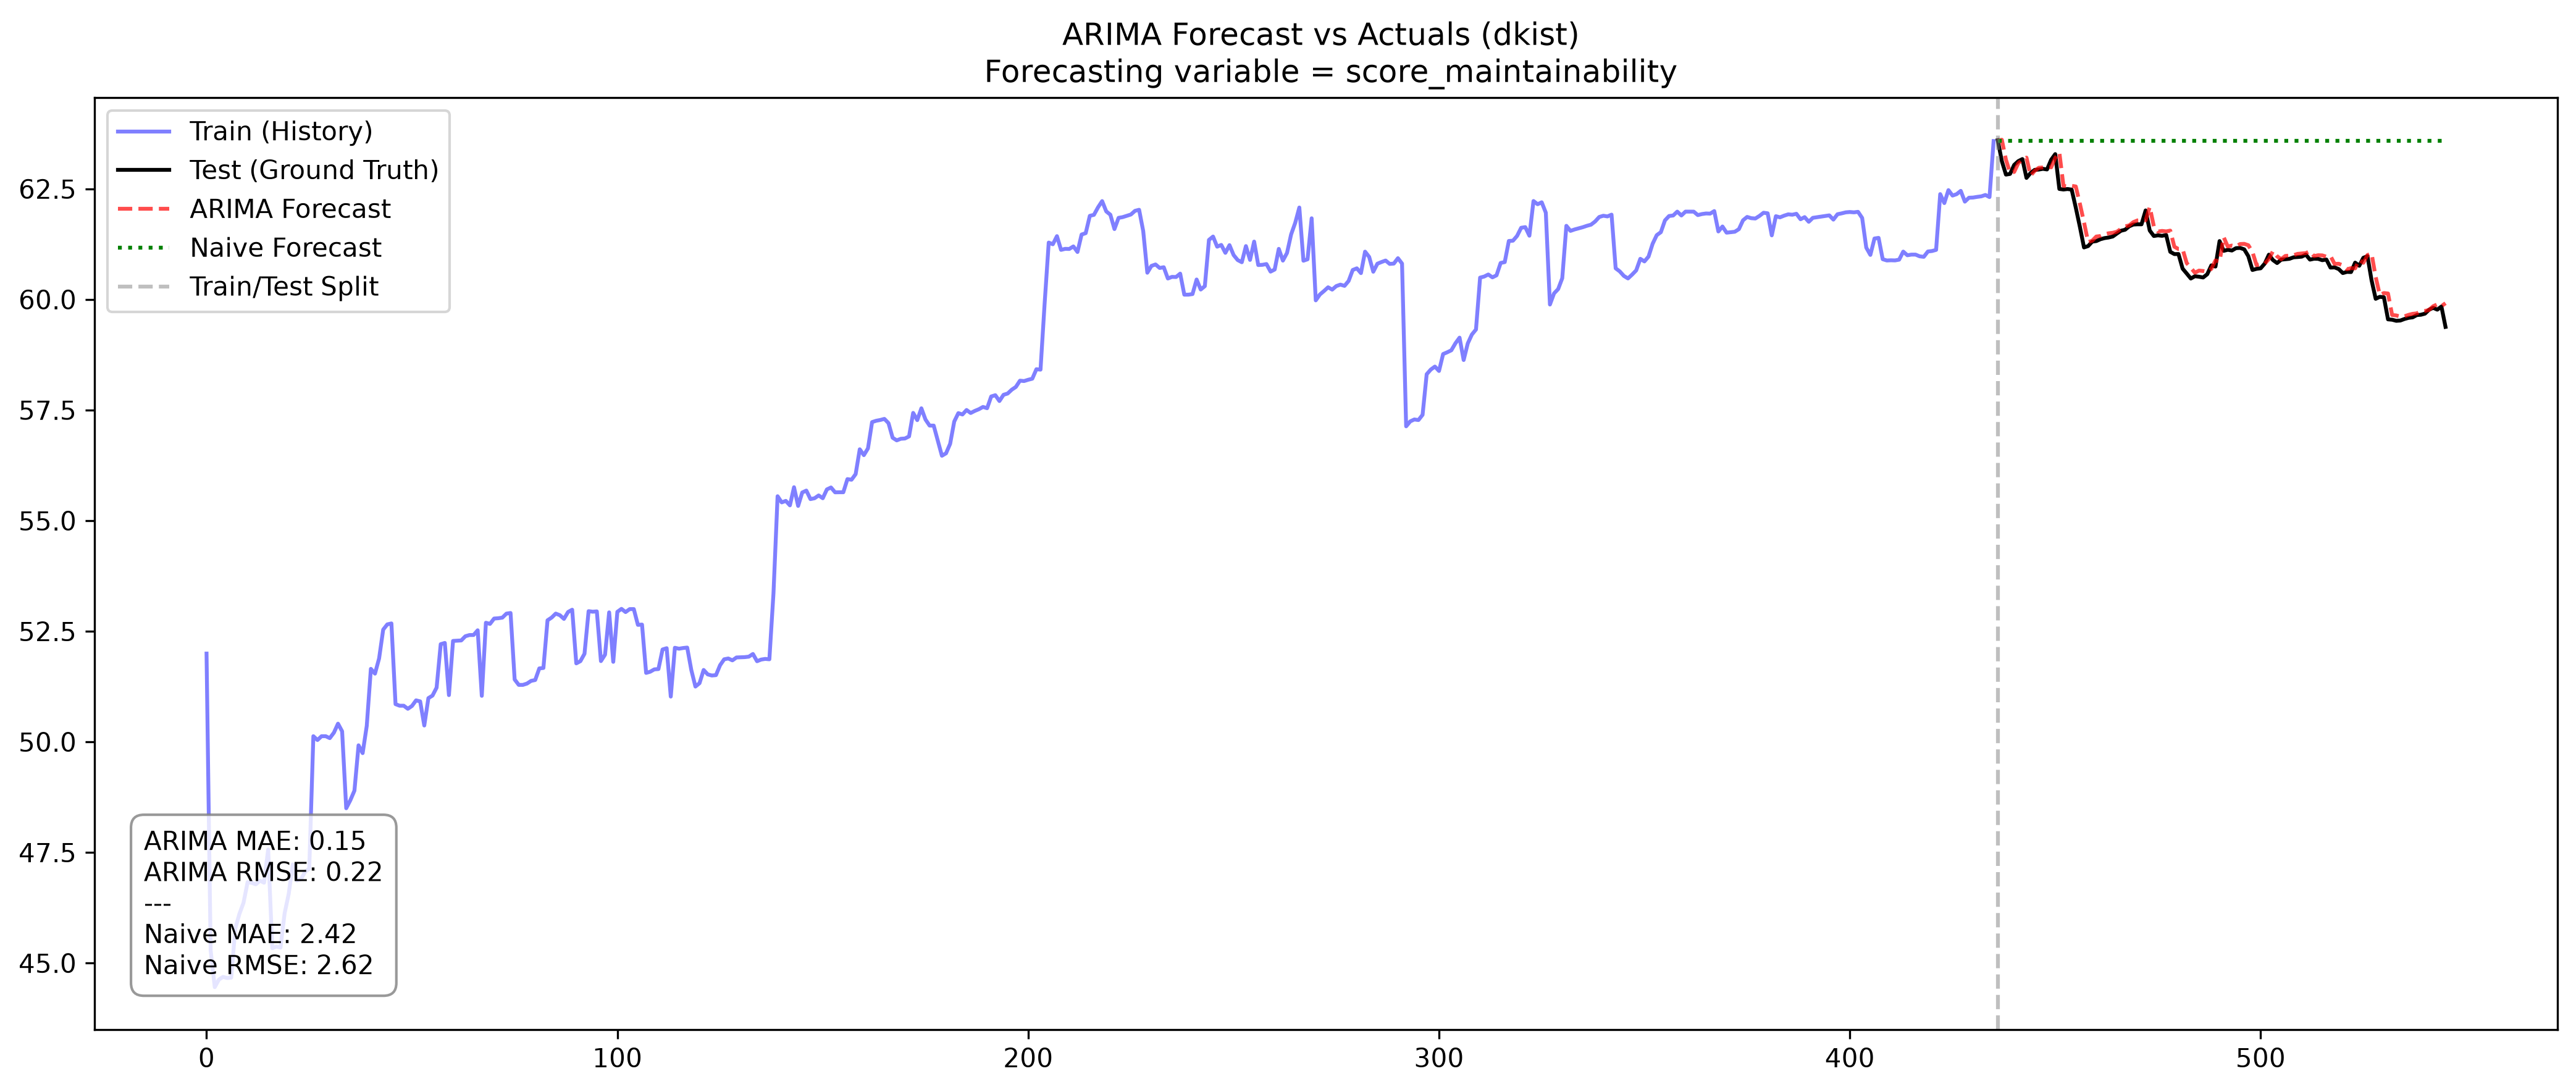
\includegraphics[width=\textwidth,height=0.40\textheight,keepaspectratio]{figures/dkist/arima-forecasting.png}
\caption{DKIST ARIMA Maintainability forecast.}
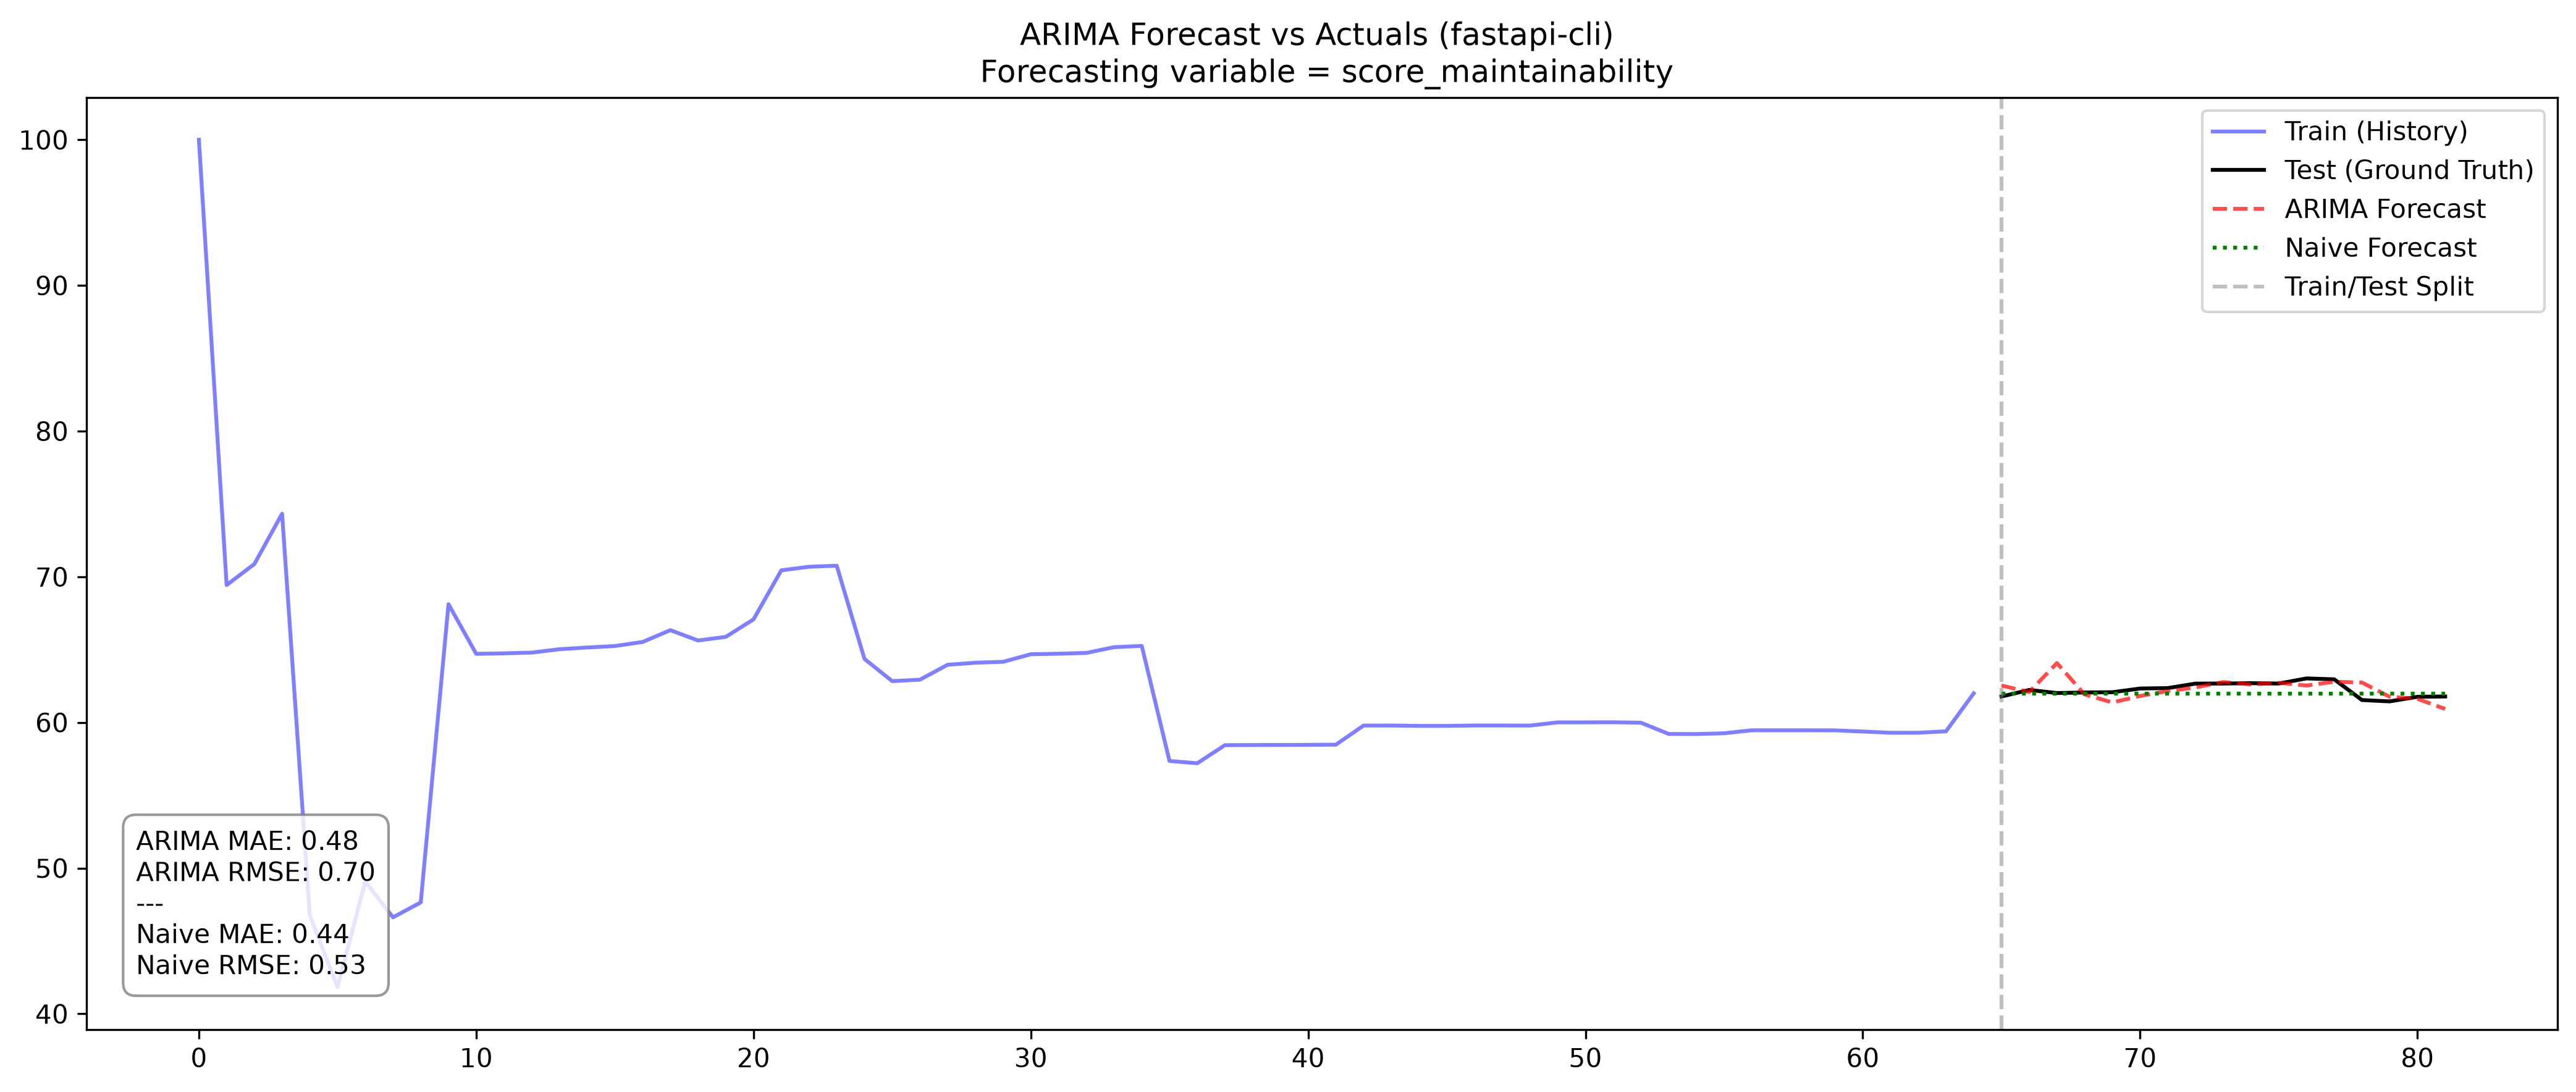
\includegraphics[width=\textwidth,height=0.40\textheight,keepaspectratio]{figures/fastapi-cli/arima-forecasting.png}
\caption*{FastAPI-cli ARIMA Maintainability forecast.}
\end{figure}

\begin{figure}[p]
\centering
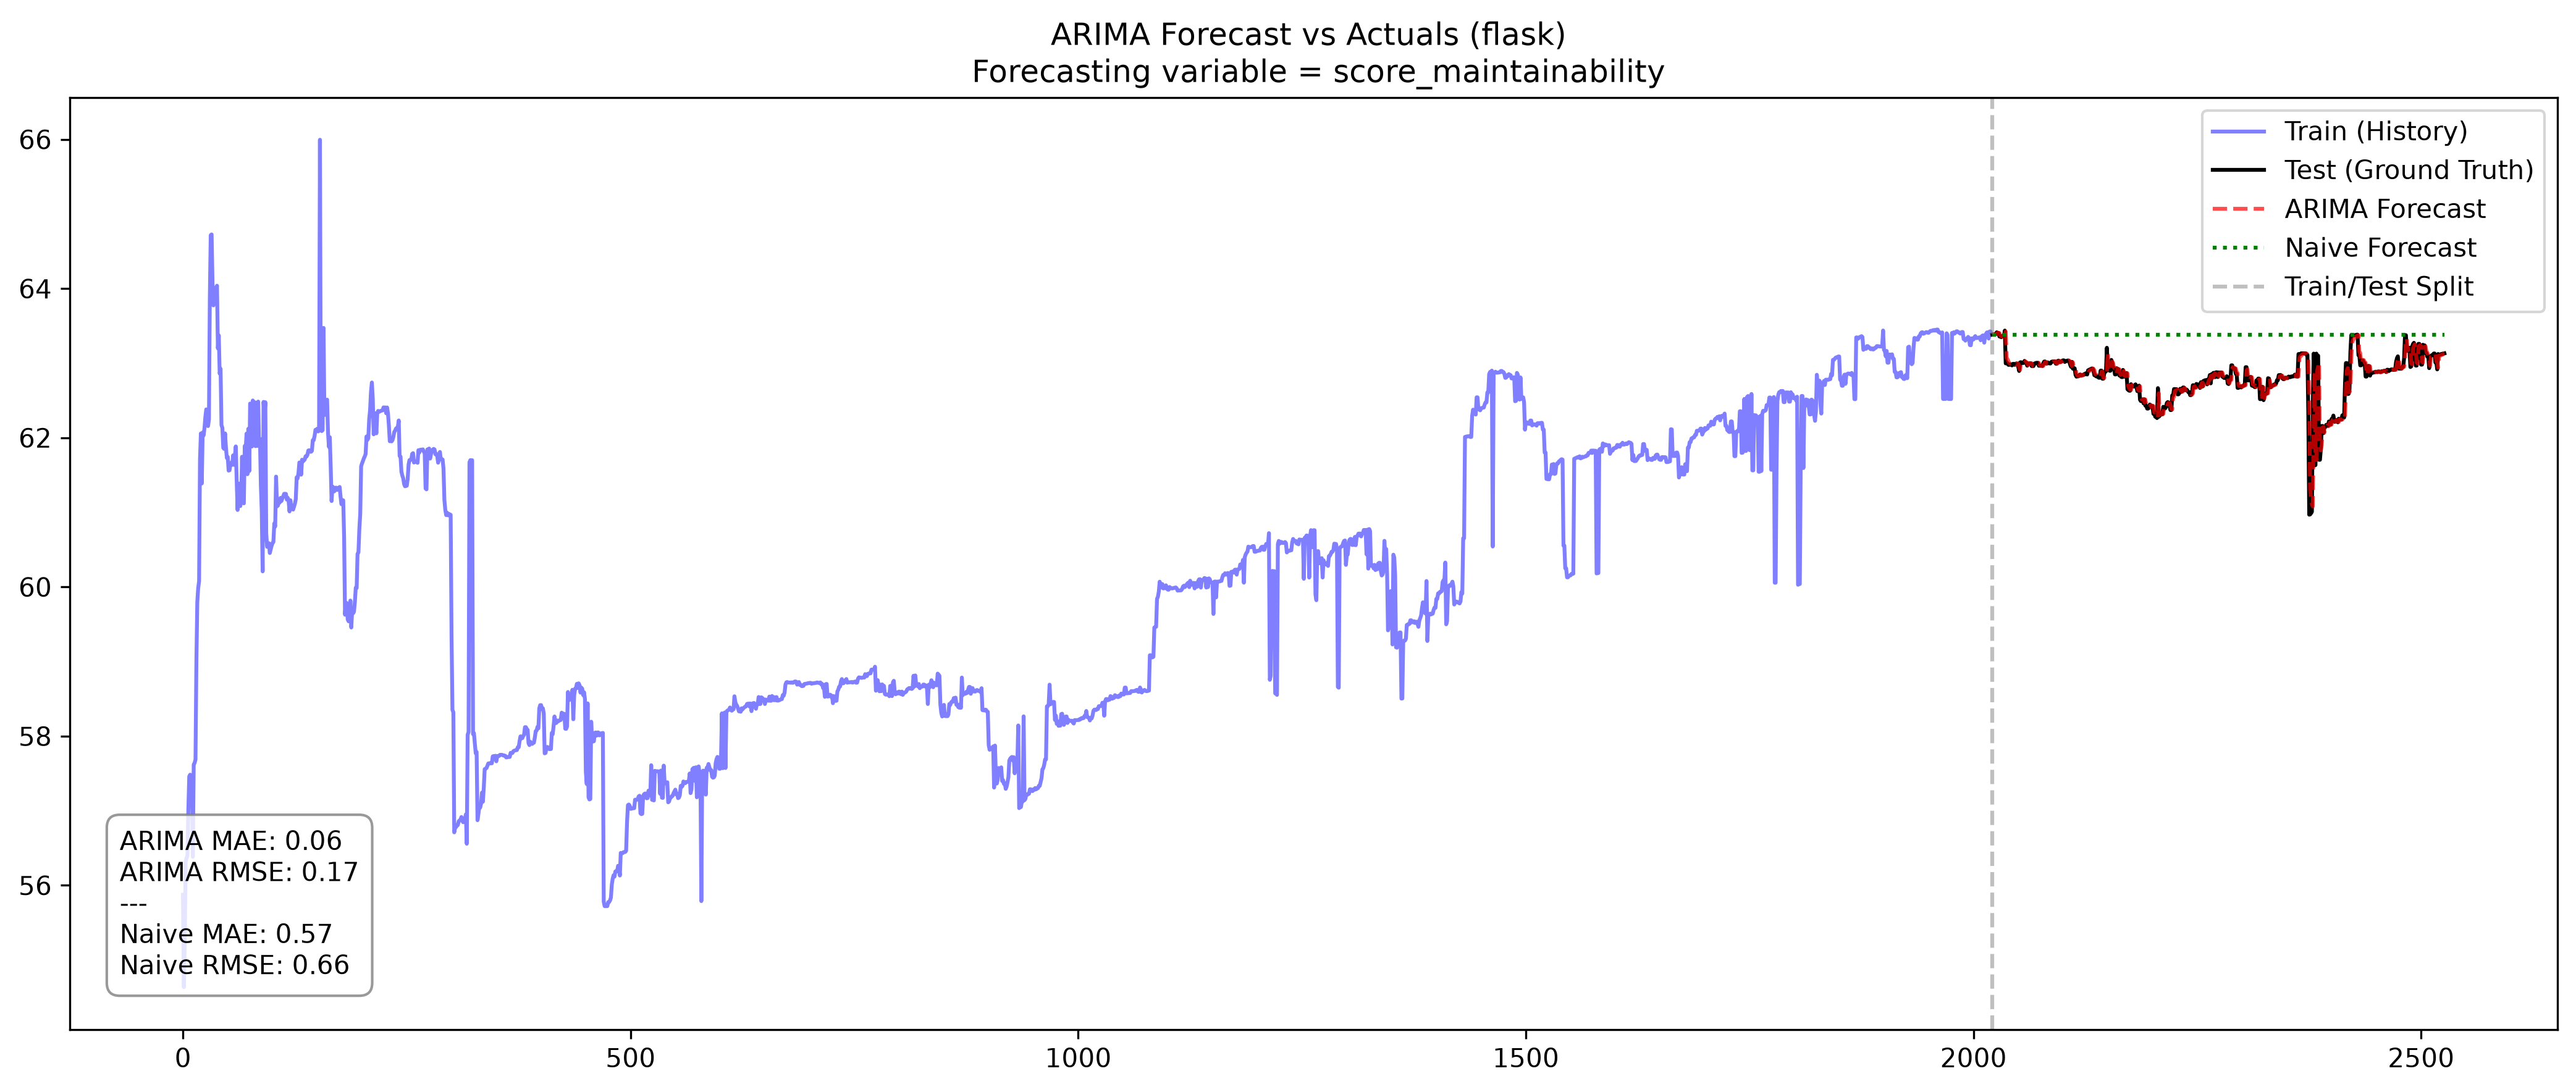
\includegraphics[width=\textwidth,height=0.40\textheight,keepaspectratio]{figures/flask/arima-forecasting.png}
\caption{Flask ARIMA Maintainability forecast.}
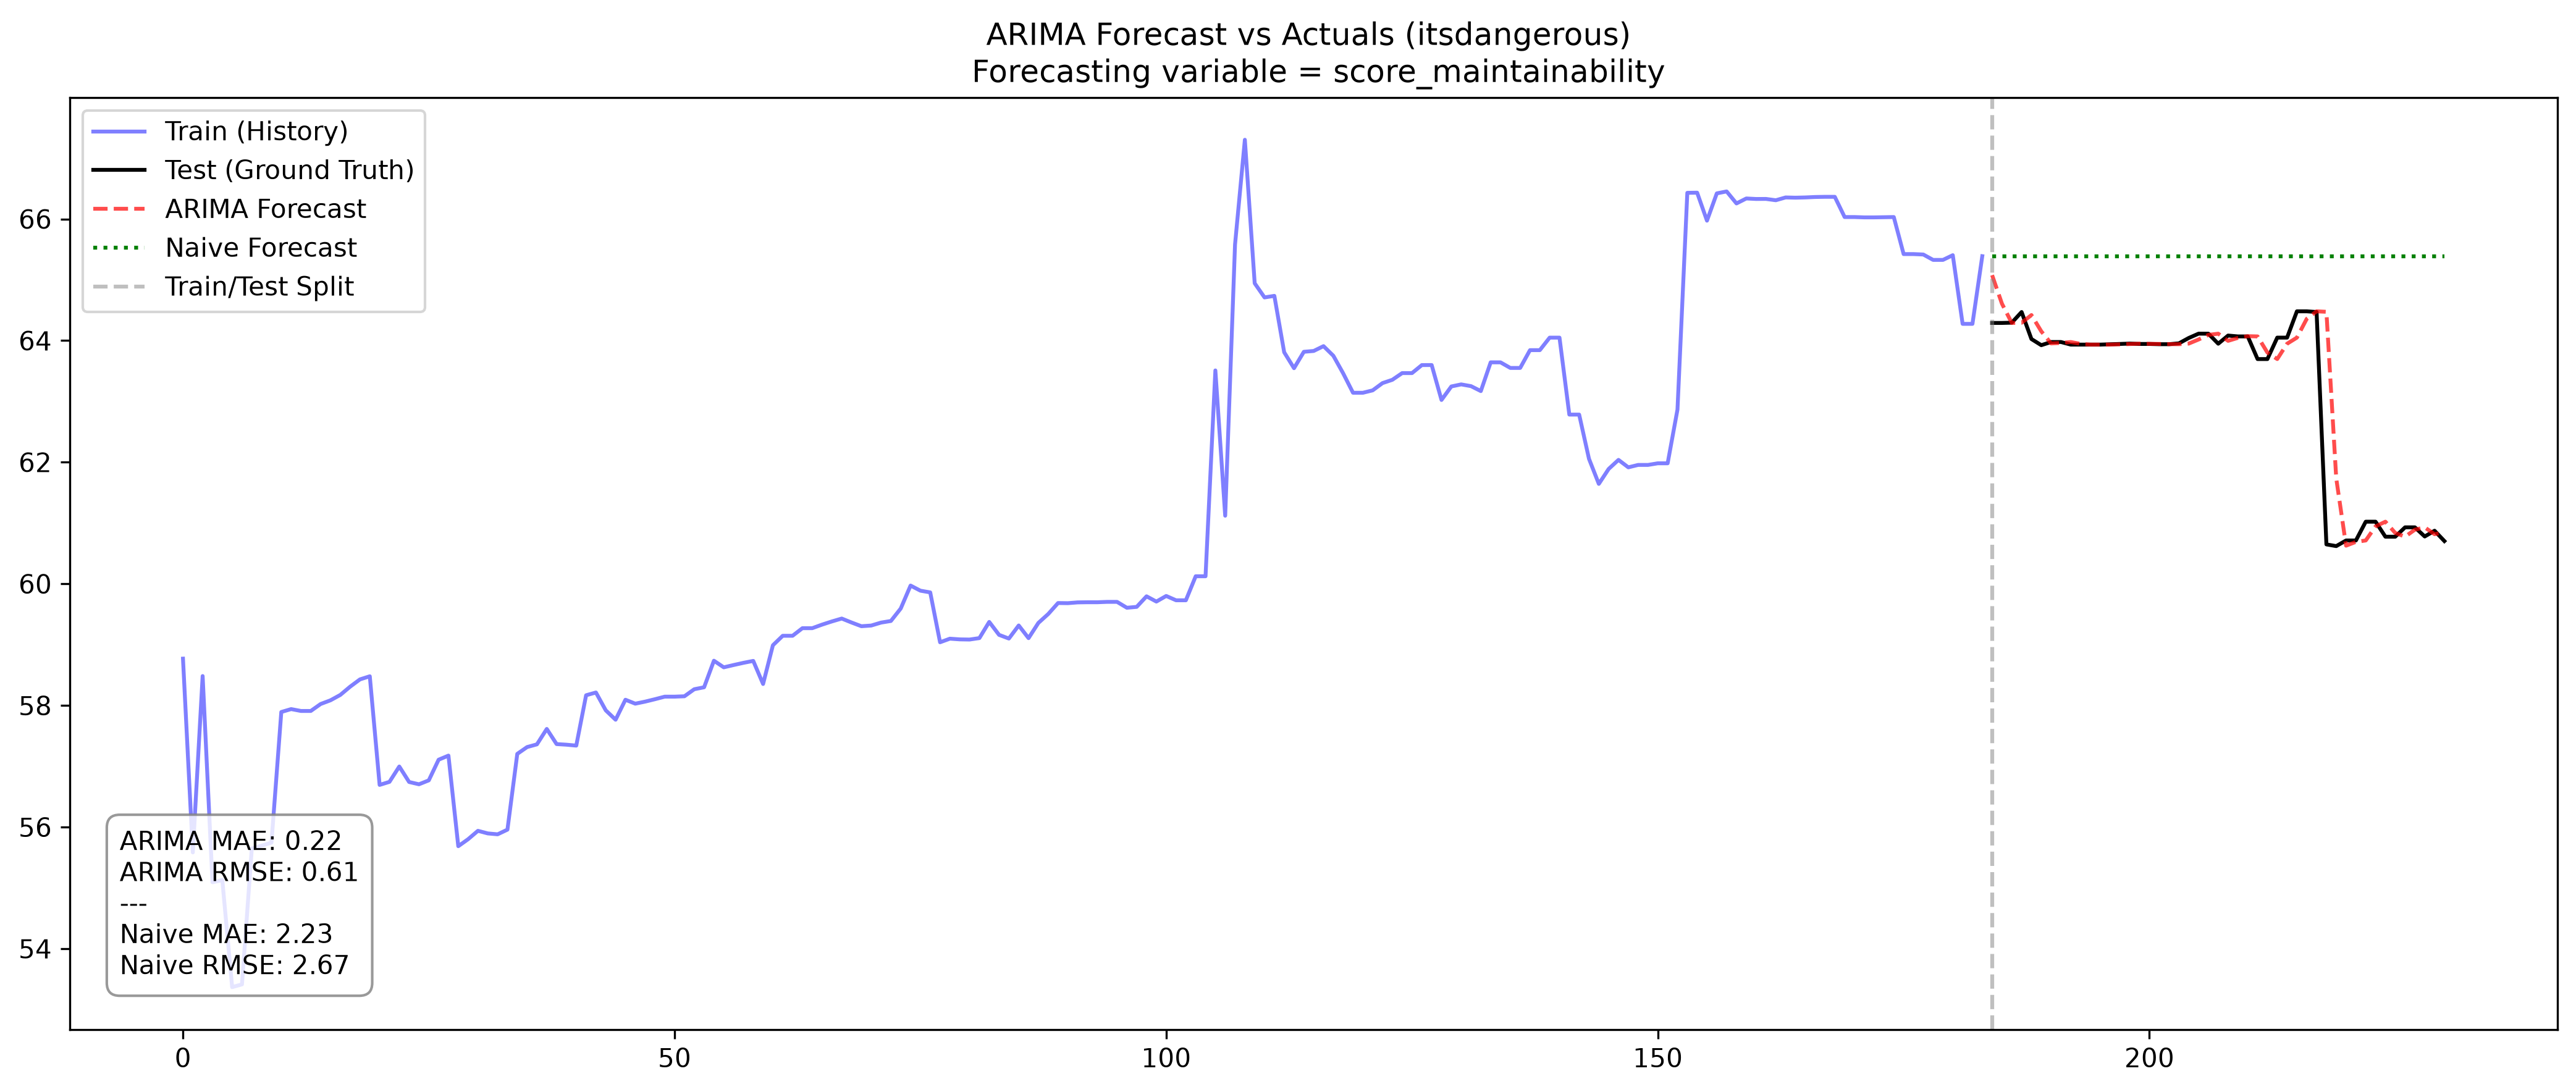
\includegraphics[width=\textwidth,height=0.40\textheight,keepaspectratio]{figures/itsdangerous/arima-forecasting.png}
\caption*{Itsdangerous ARIMA Maintainability forecast.}
\end{figure}

\begin{figure}[p]
\centering
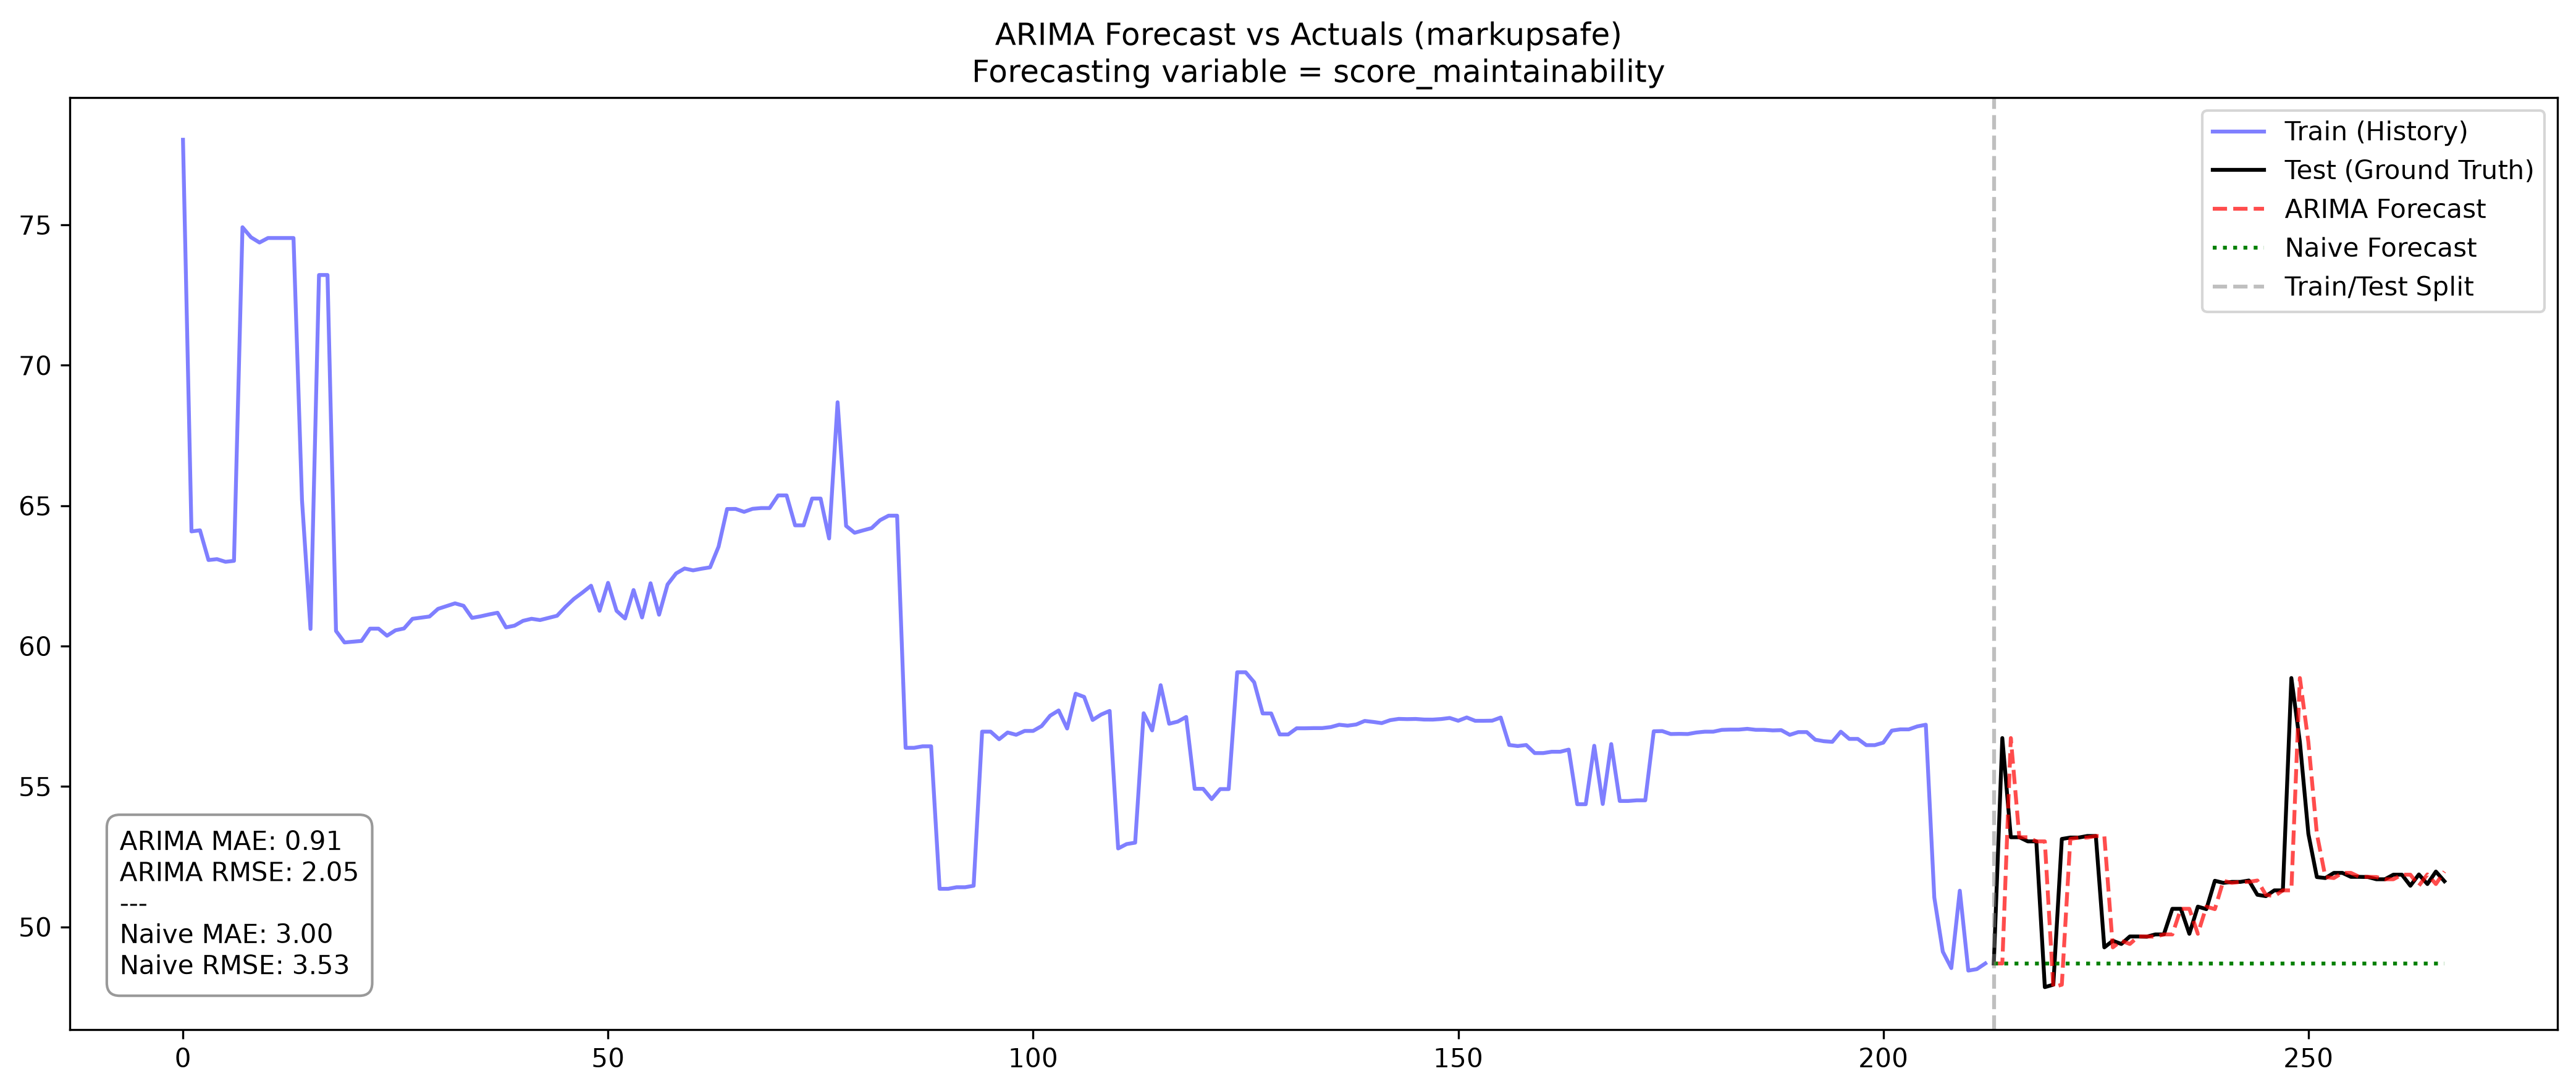
\includegraphics[width=\textwidth,height=0.40\textheight,keepaspectratio]{figures/markupsafe/arima-forecasting.png}
\caption{Markupsafe ARIMA Maintainability forecast.}
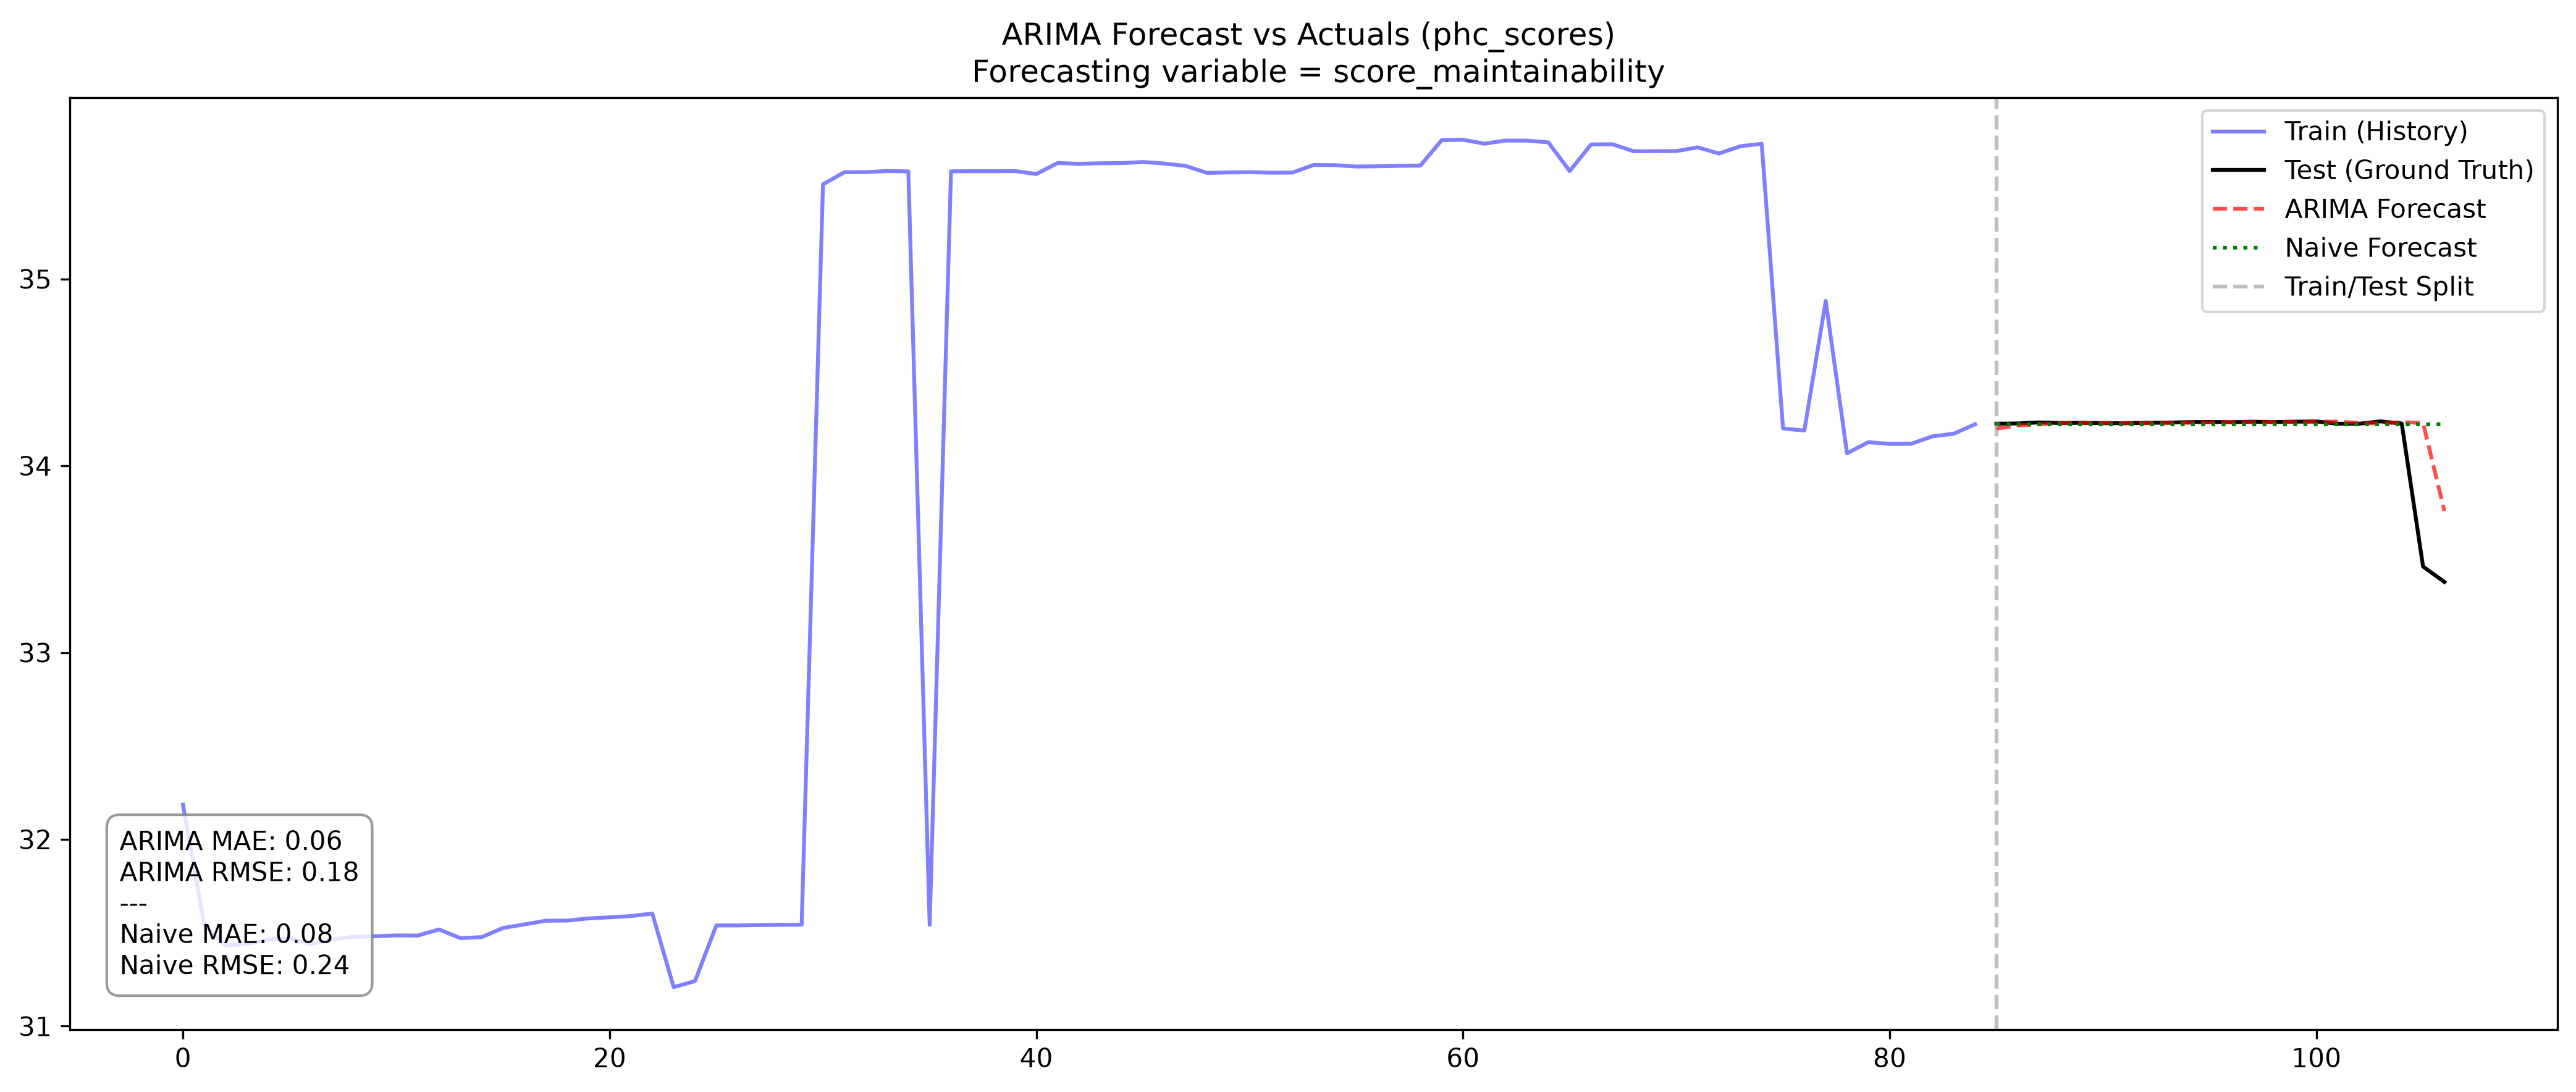
\includegraphics[width=\textwidth,height=0.40\textheight,keepaspectratio]{figures/phc_scores/arima-forecasting.png}
\caption*{PHC ARIMA Maintainability forecast.}
\end{figure}

\begin{figure}[p]
\centering
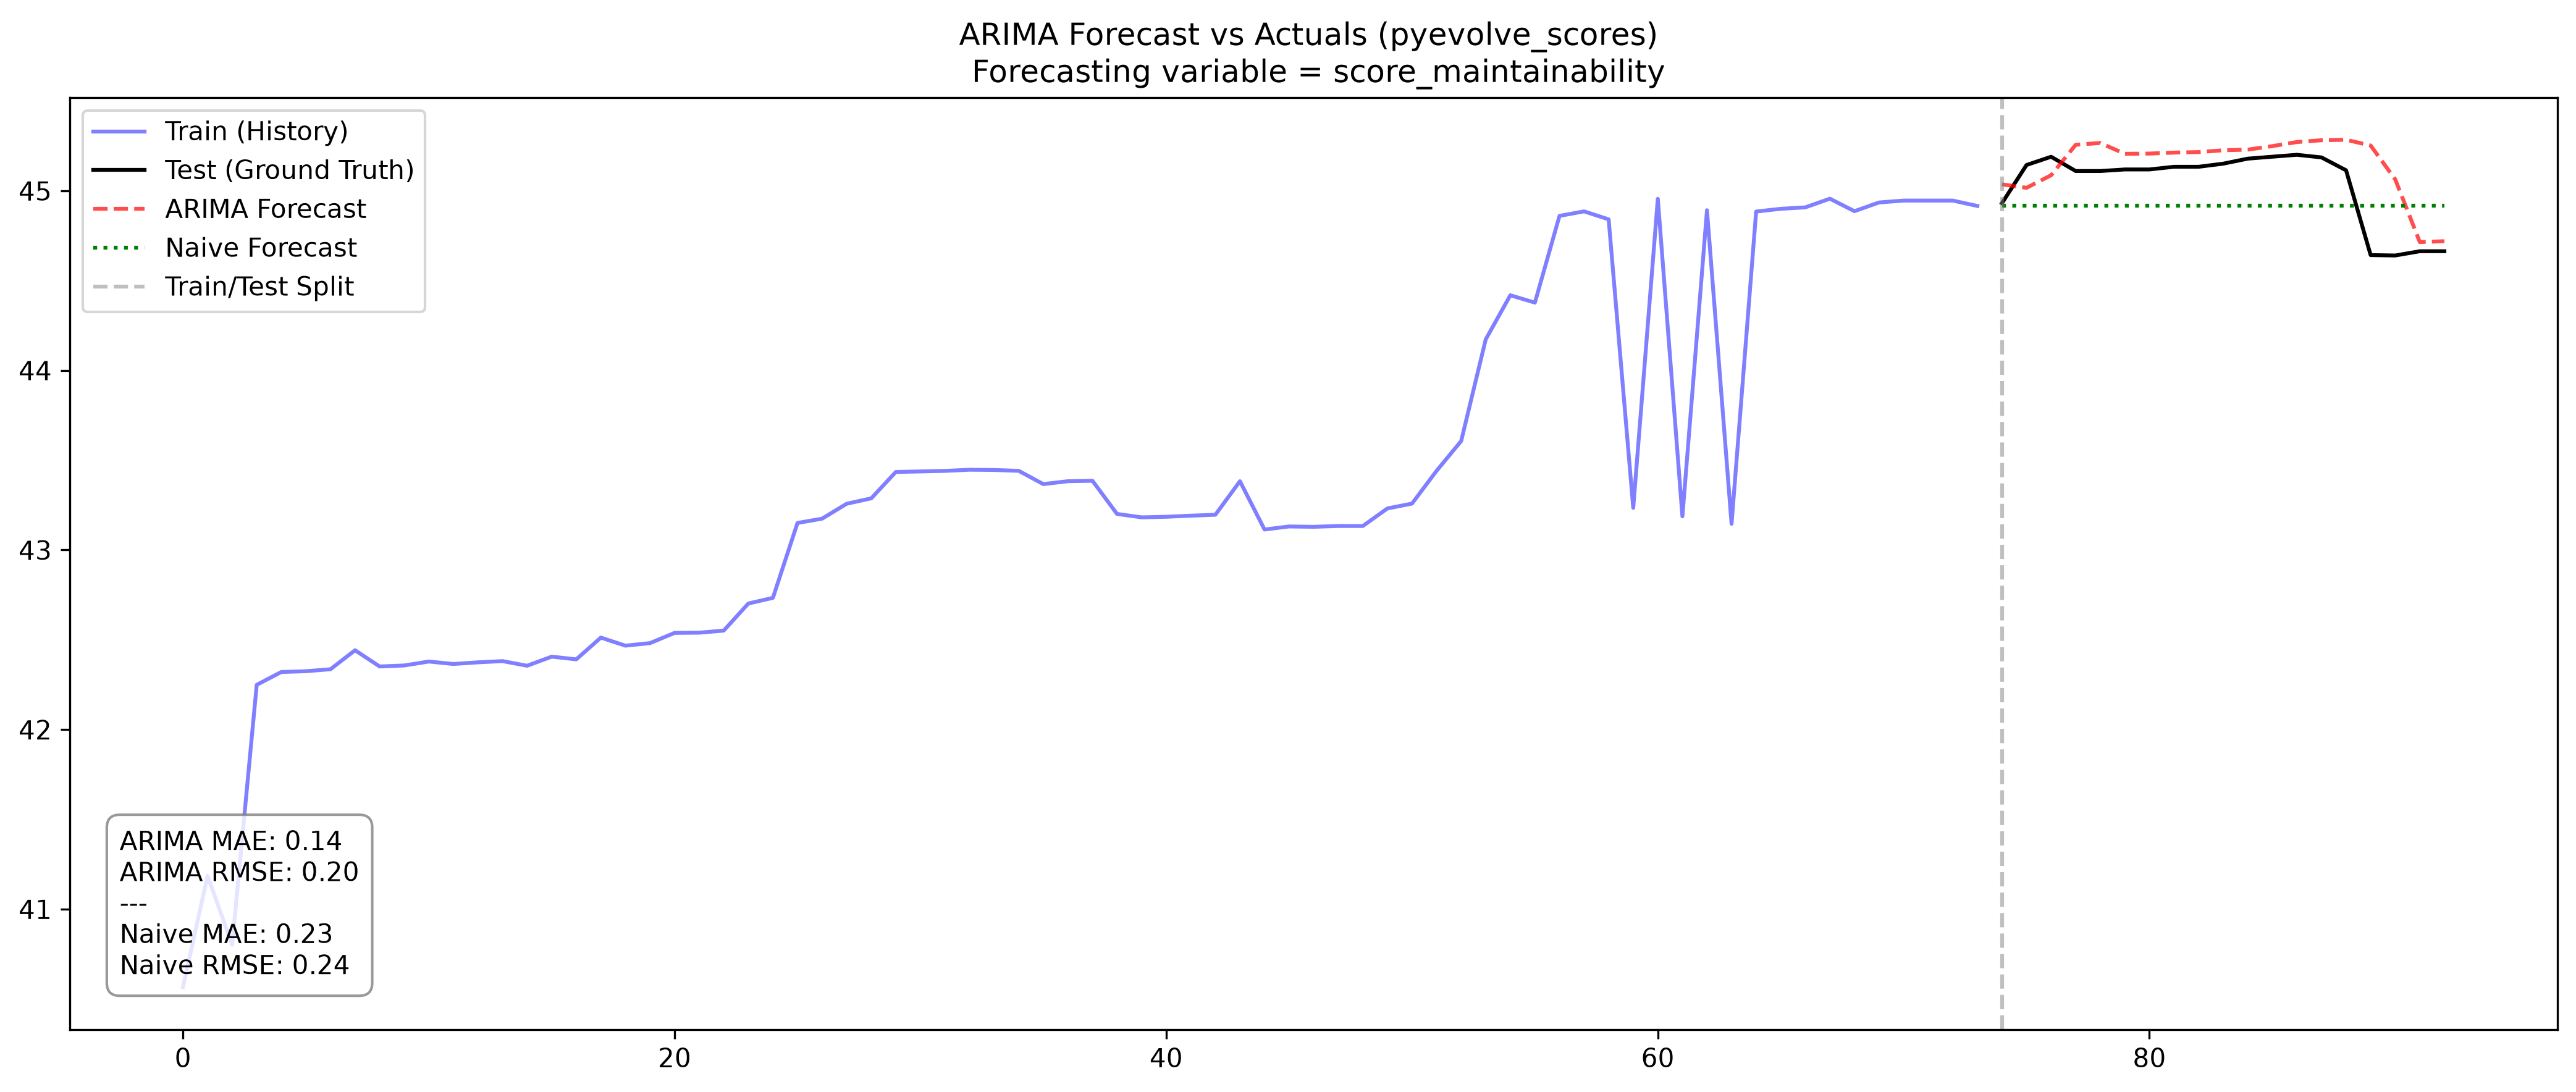
\includegraphics[width=\textwidth,height=0.40\textheight,keepaspectratio]{figures/pyevolve_scores/arima-forecasting.png}
\caption{Pyevolve ARIMA Maintainability forecast.}
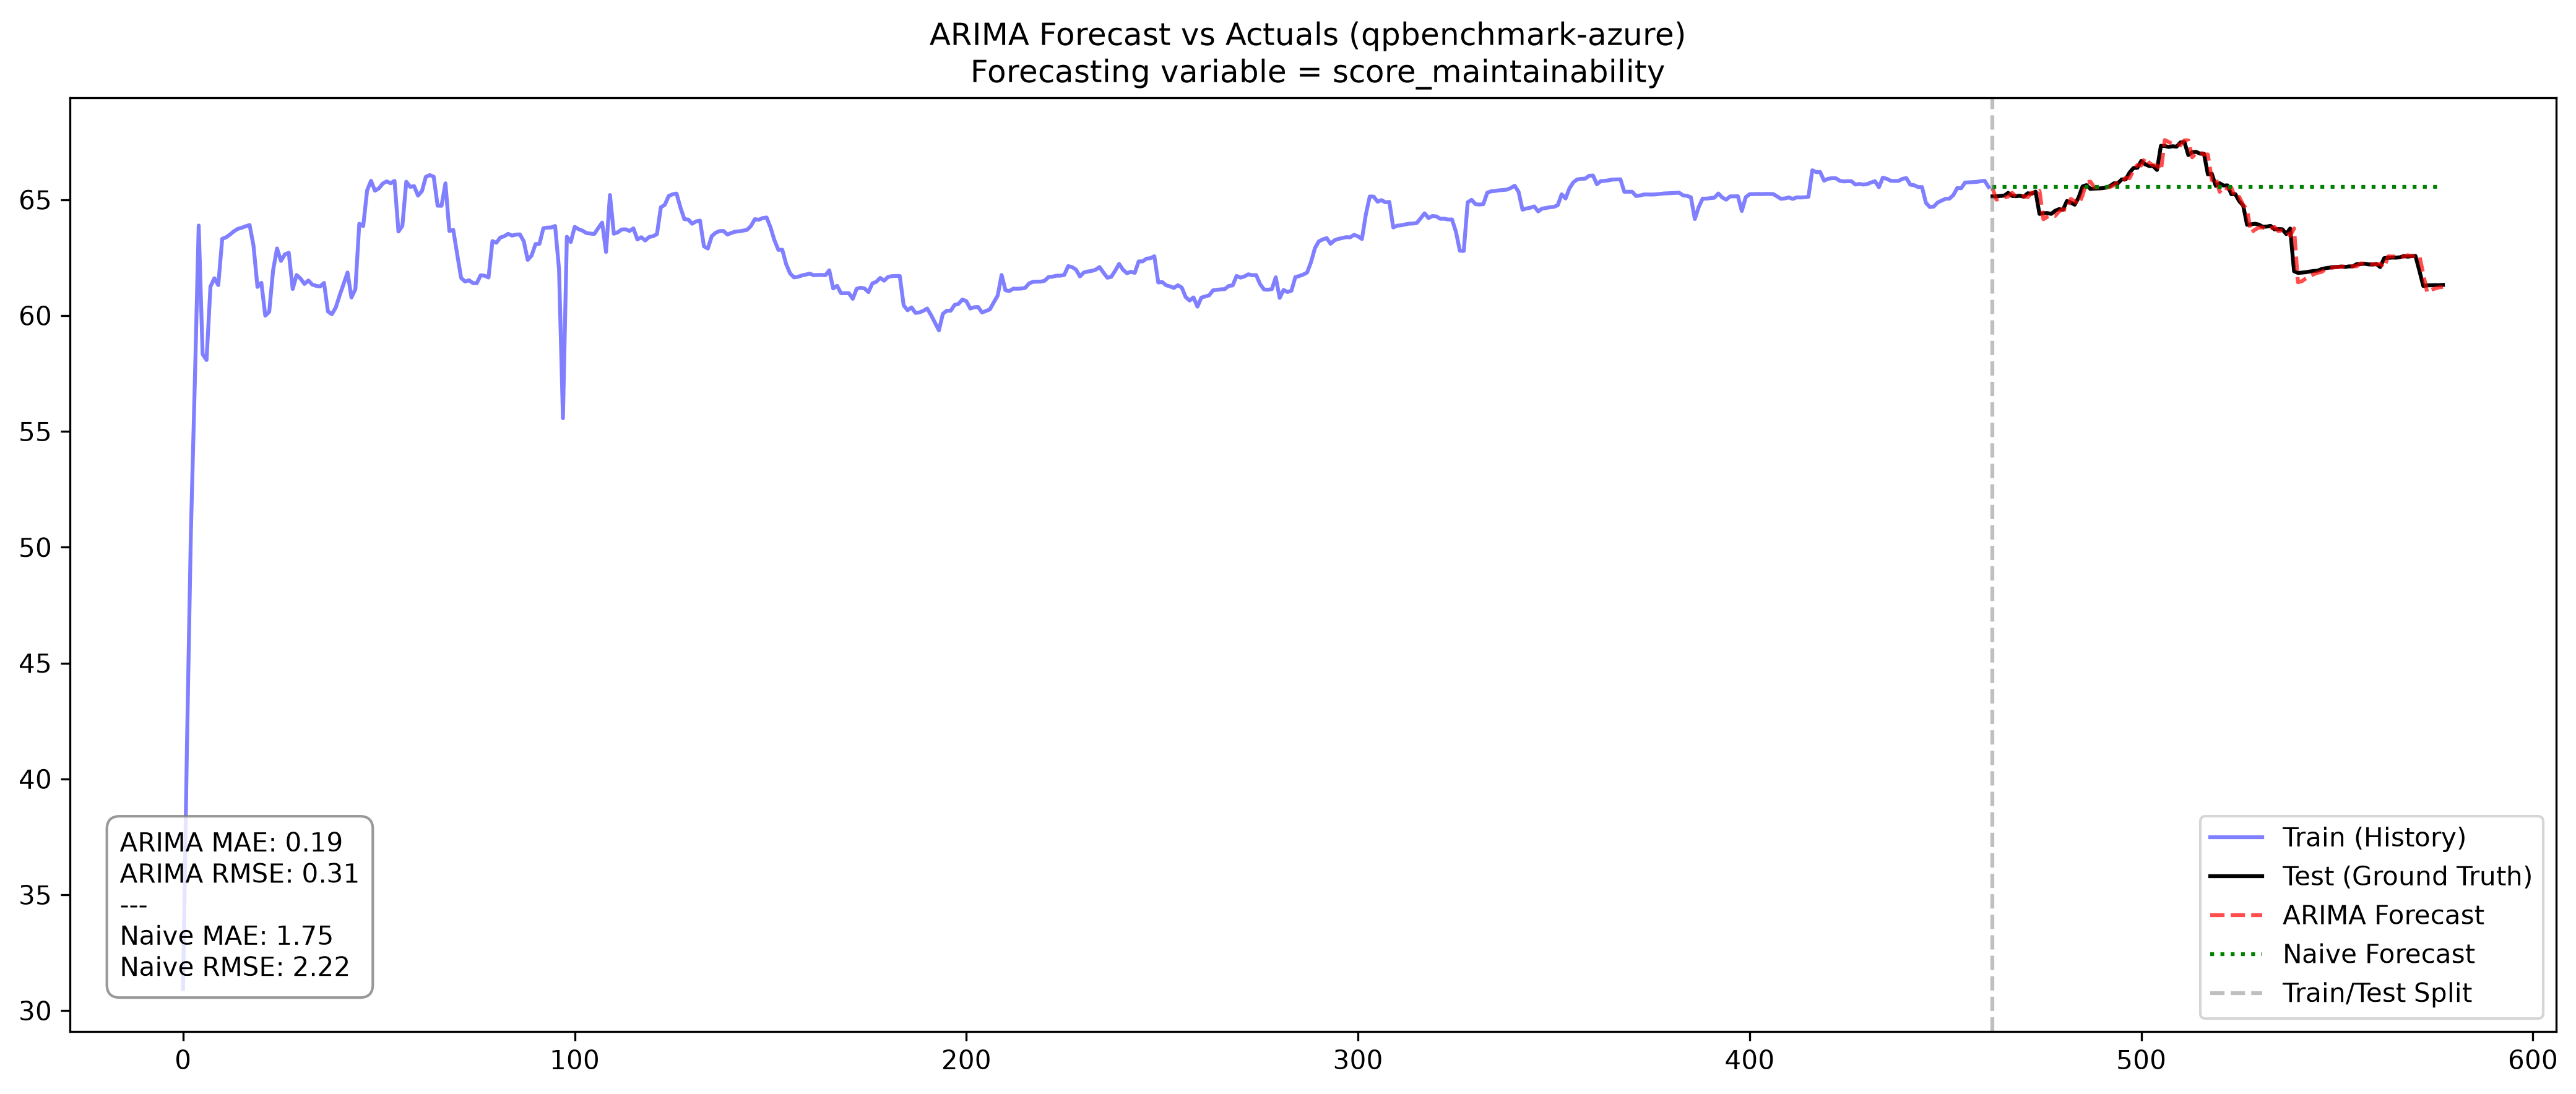
\includegraphics[width=\textwidth,height=0.40\textheight,keepaspectratio]{figures/qpbenchmark-azure/arima-forecasting.png}
\caption*{qpbenchmark ARIMA Maintainability forecast.}
\end{figure}

\begin{figure}[p]
\centering
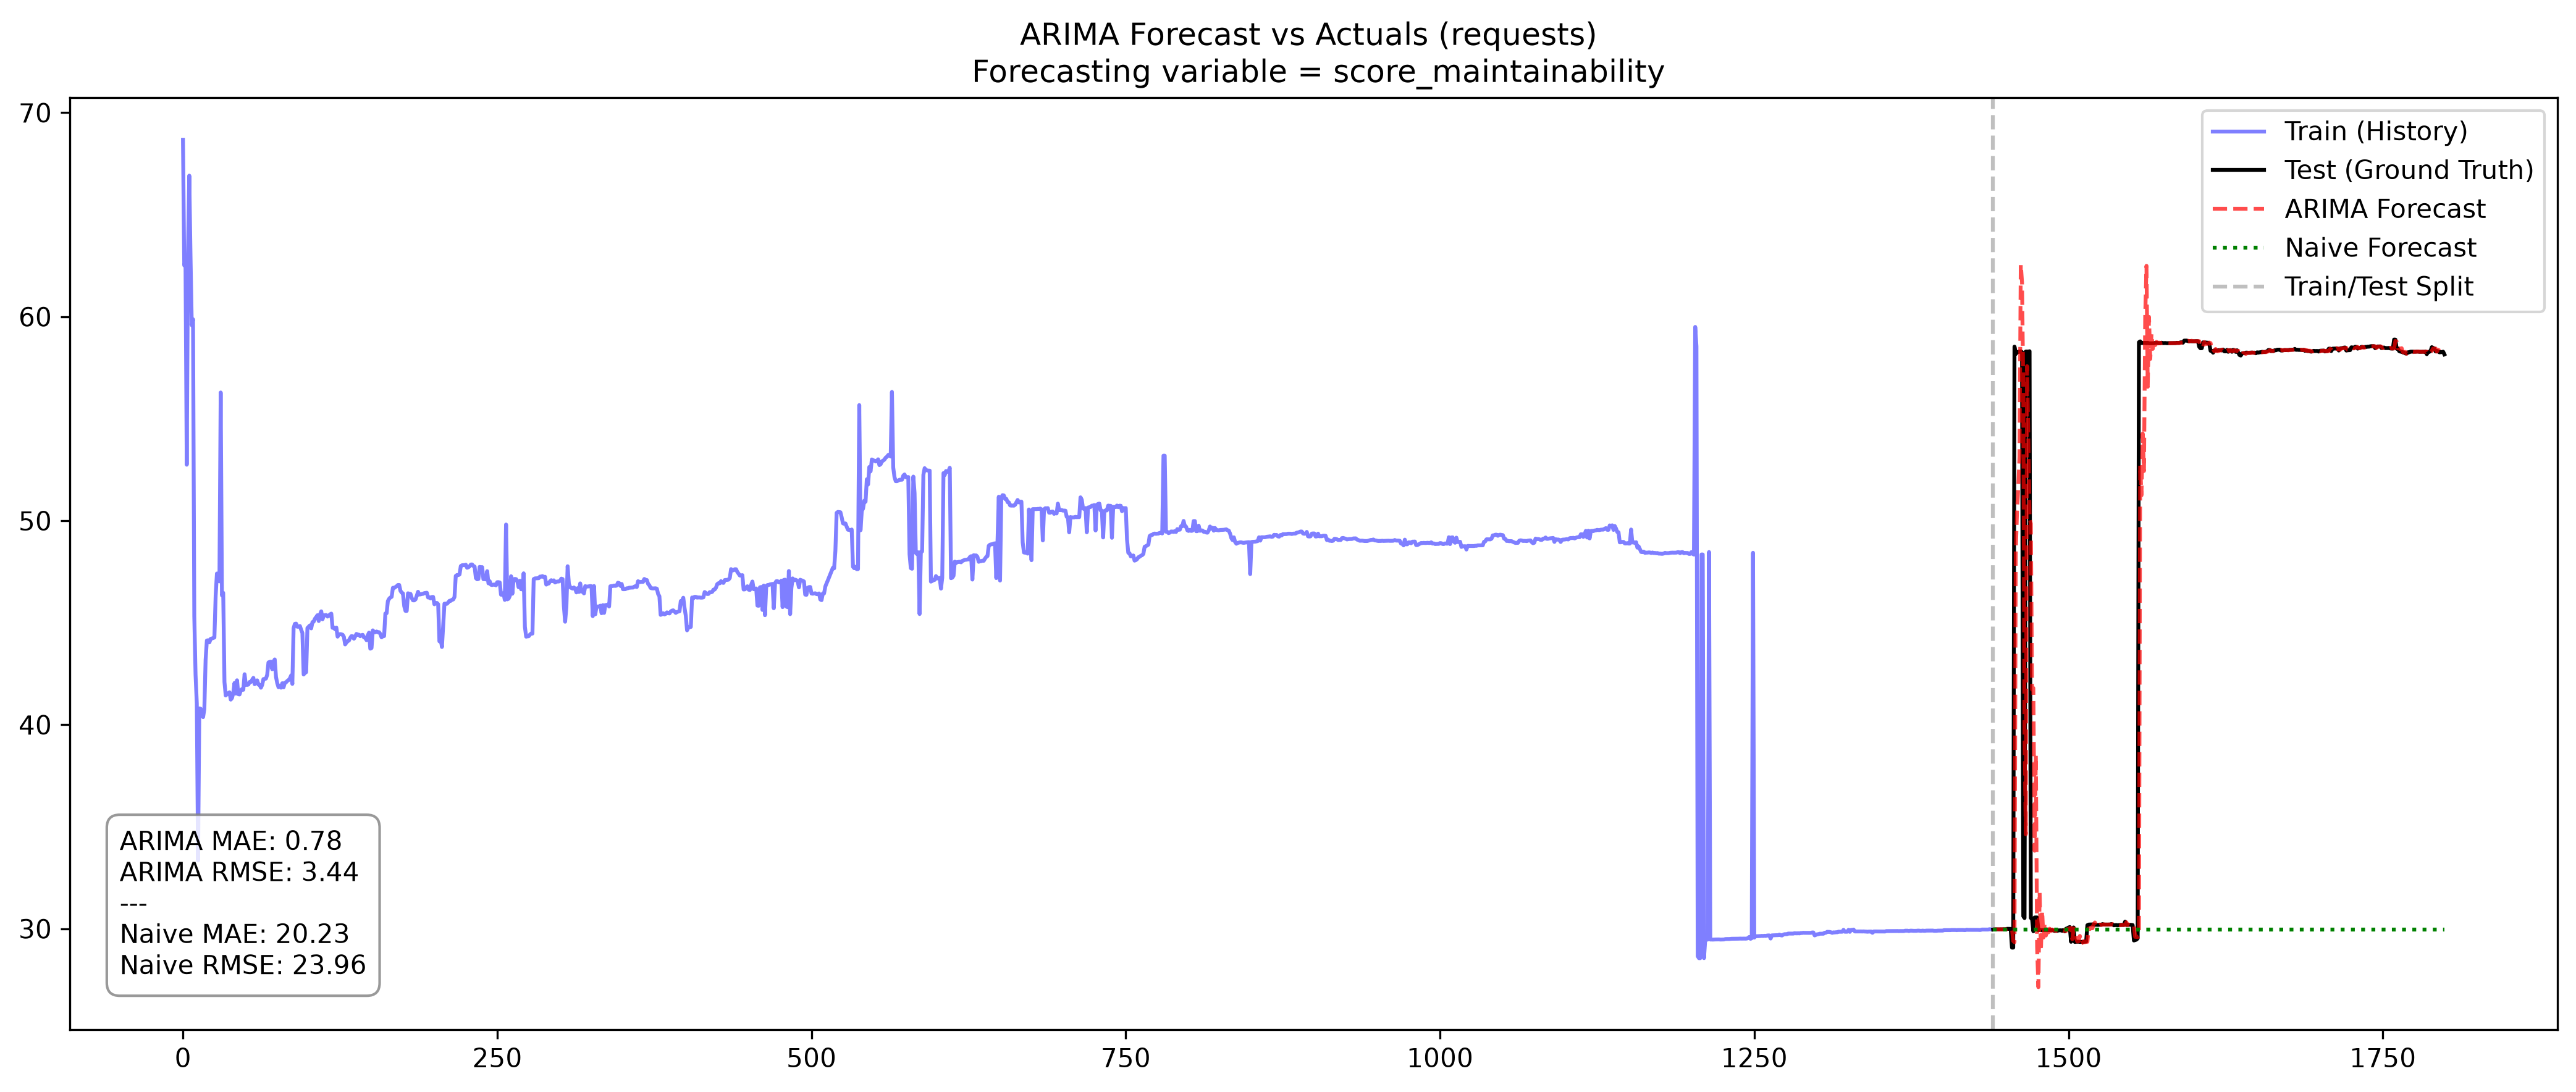
\includegraphics[width=\textwidth,height=0.40\textheight,keepaspectratio]{figures/requests/arima-forecasting.png}
\caption{Requests ARIMA Maintainability forecast.}
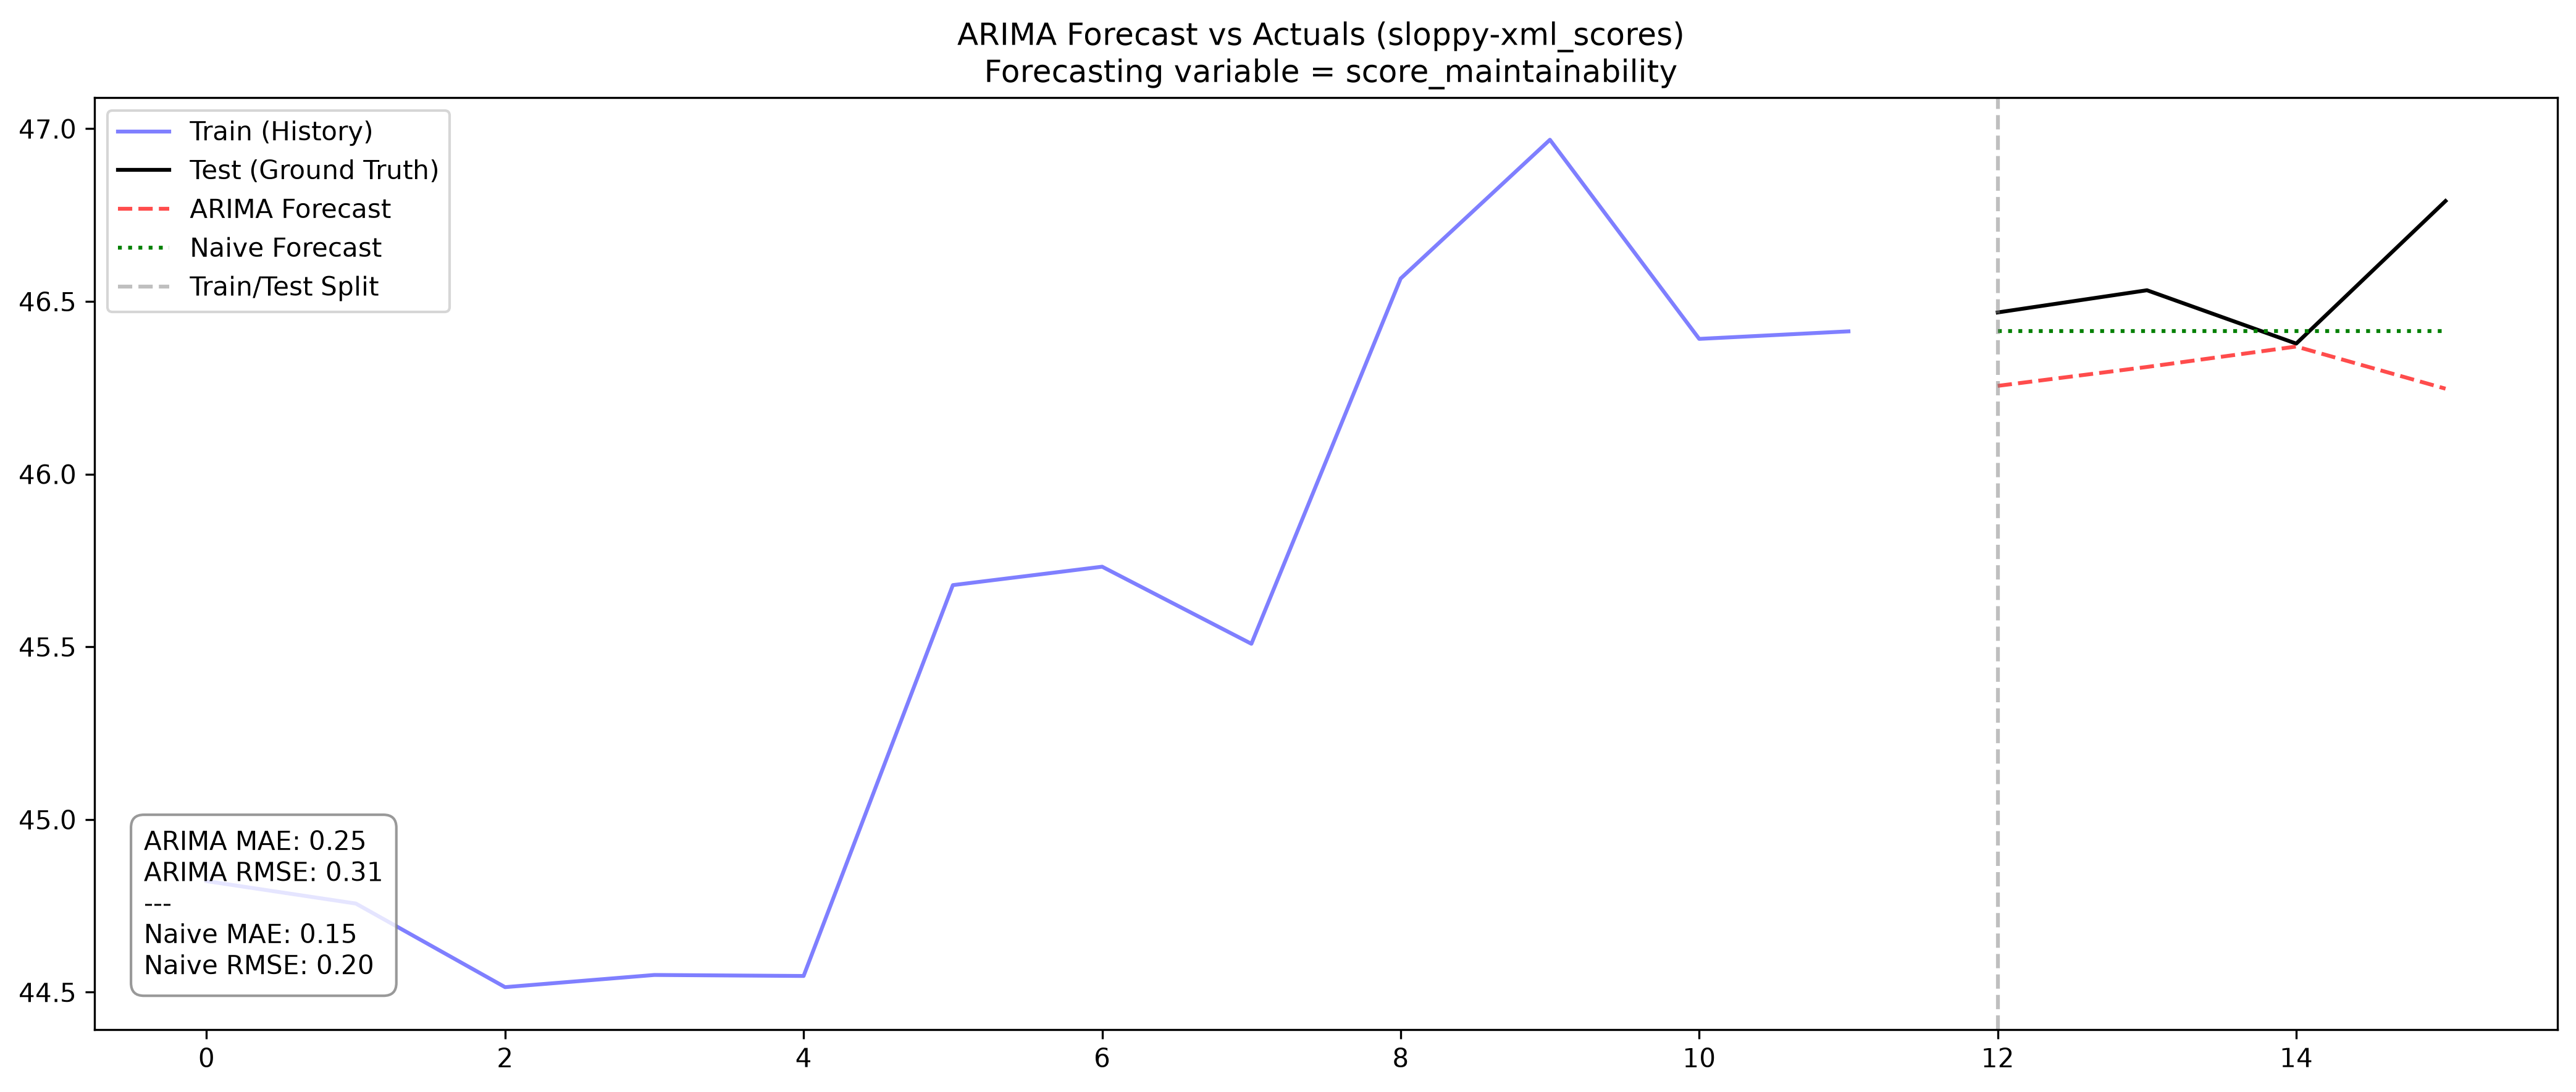
\includegraphics[width=\textwidth,height=0.40\textheight,keepaspectratio]{figures/sloppy-xml_scores/arima-forecasting.png}
\caption*{Sloppy-xml-py ARIMA Maintainability forecast.}
\end{figure}

\begin{figure}[p]
\centering
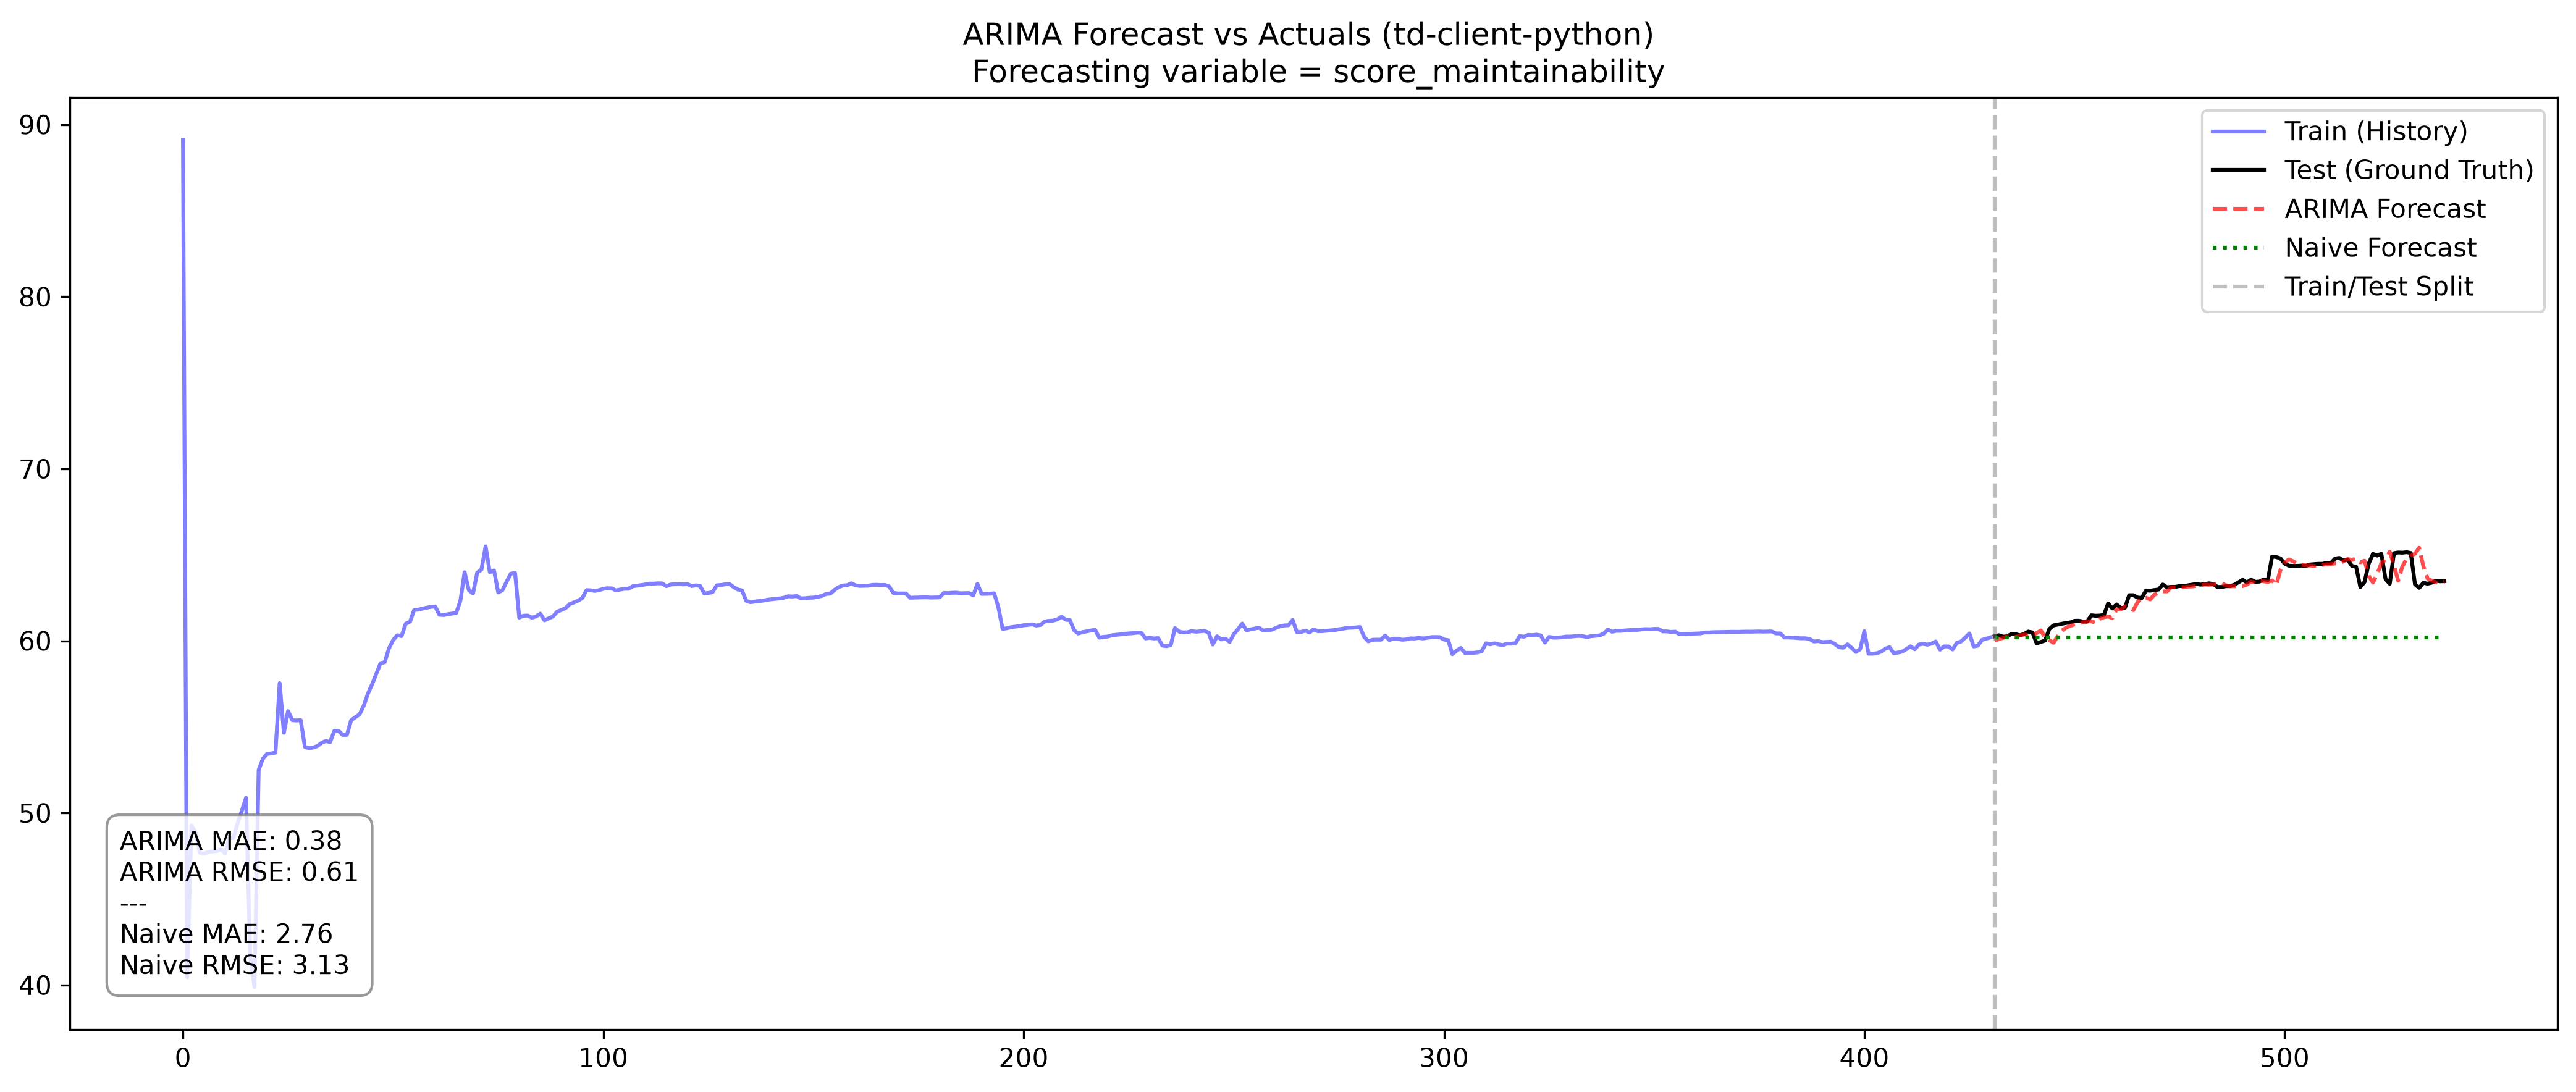
\includegraphics[width=\textwidth,height=0.40\textheight,keepaspectratio]{figures/td-client-python/arima-forecasting.png}
\caption{Td-client-python ARIMA Maintainability forecast.}
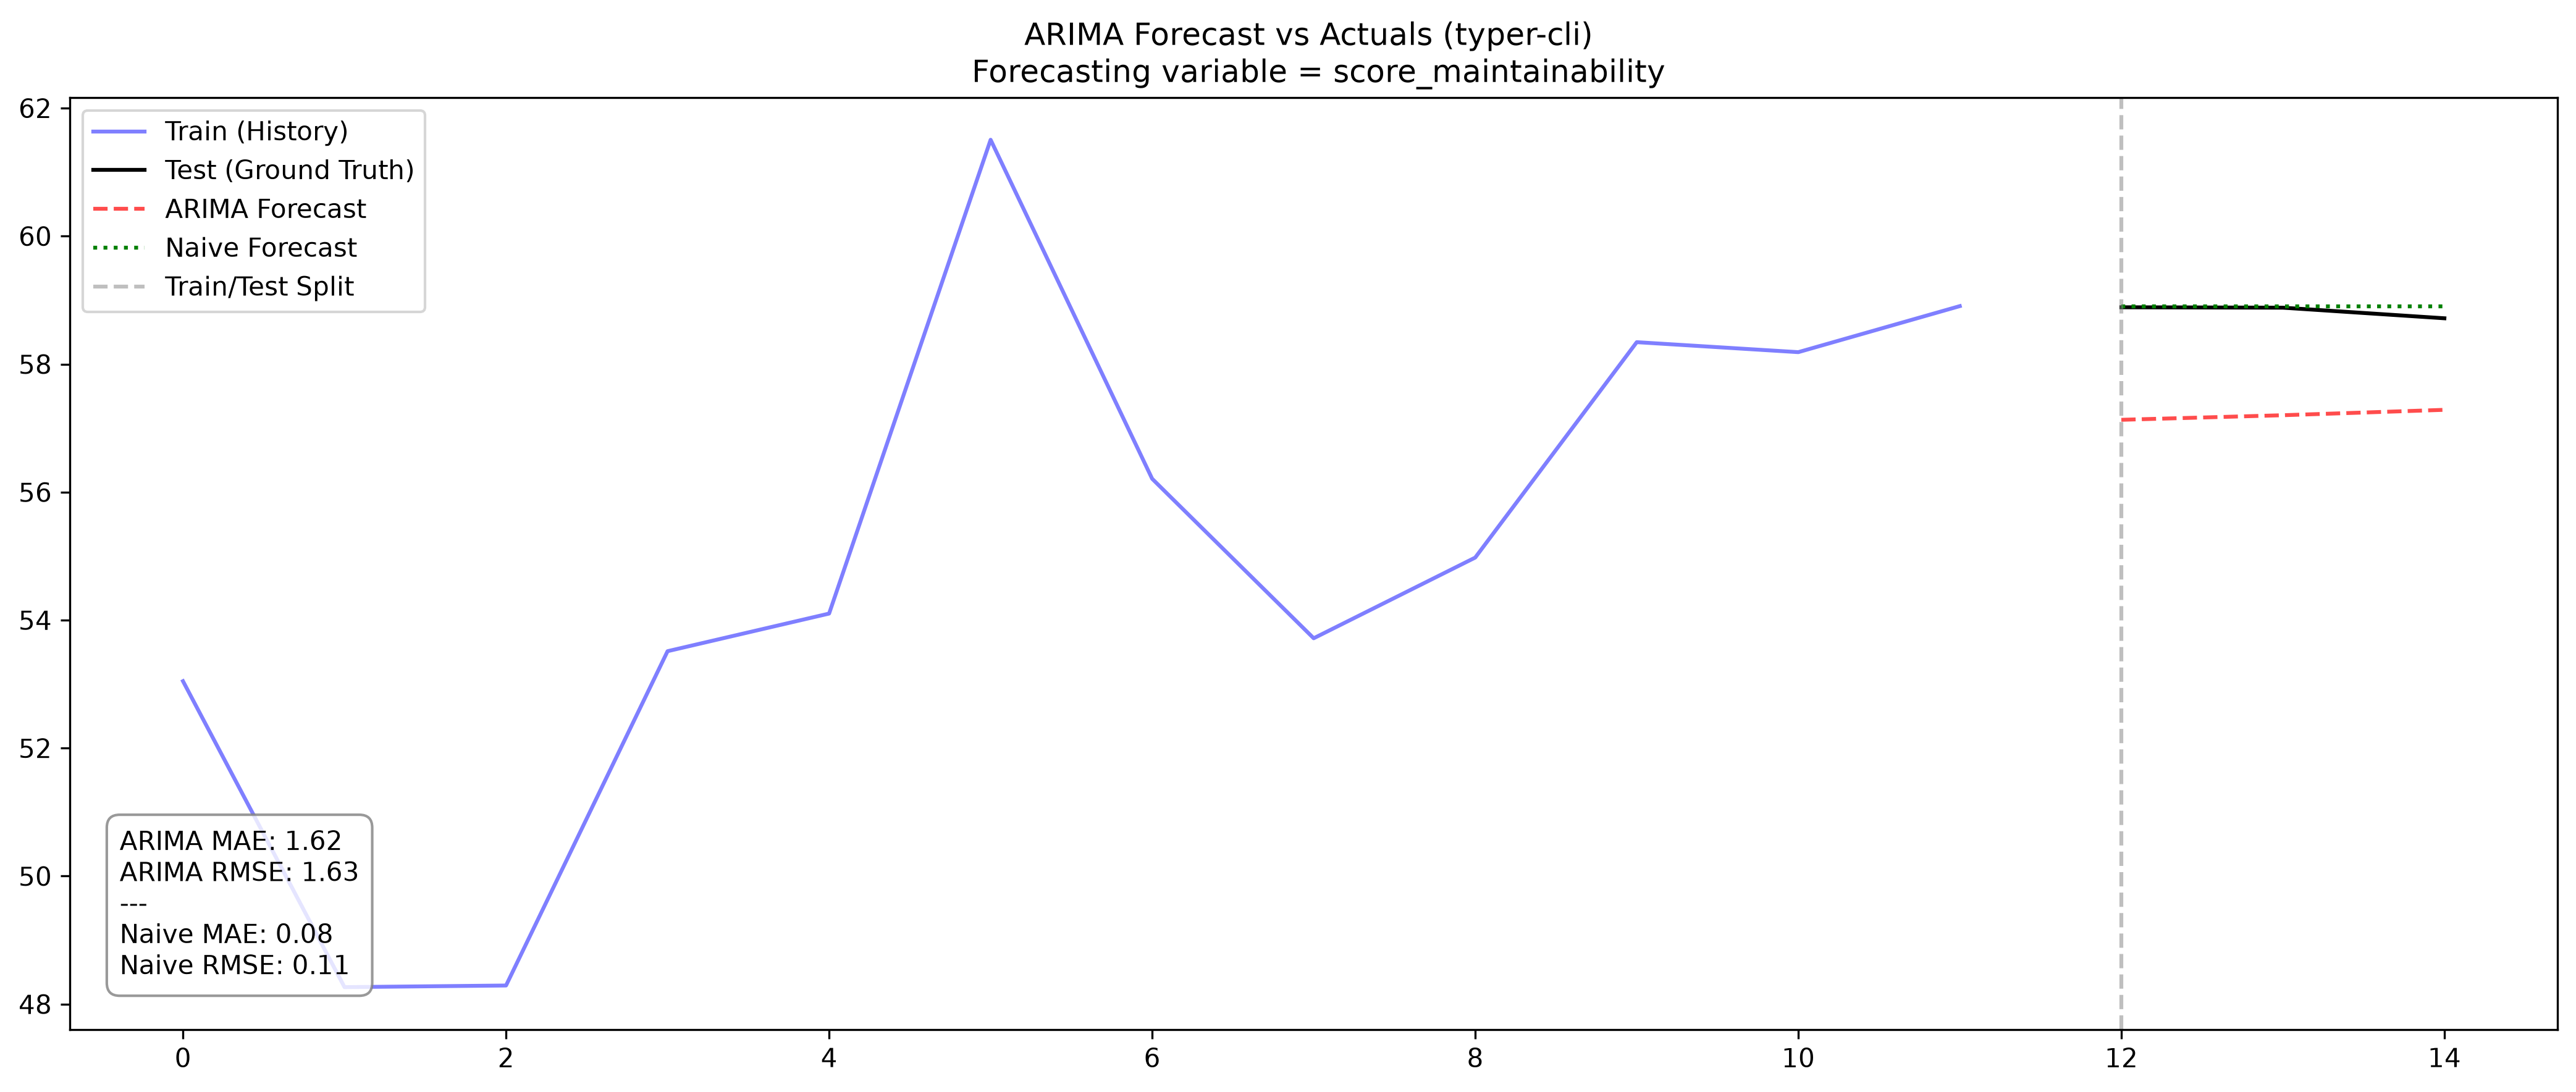
\includegraphics[width=\textwidth,height=0.40\textheight,keepaspectratio]{figures/typer-cli/arima-forecasting.png}
\caption*{Typer-cli ARIMA Maintainability forecast.}
\end{figure}

\clearpage
\phantomsection
\addcontentsline{toc}{chapter}{References}
\renewcommand{\bibname}{References}
\bibliographystyle{plainnat}
\bibliography{references}



\end{document}
